% Incognita paper P008. Rules: AGENTS.md, section 5; docs/writing.md (template preamble; at most
% 100 pages). Working notes go in notebook/, never in this file; what serves only the referees and
% the owner is in DOSSIER.md.
% One source, two builds (AGENTS.md 5.2), after `python3 scripts/certify.py bib`:
%   reader:    latexmk -pdf -interaction=nonstopmode -halt-on-error -cd papers/P008-transfer-lower-bound/paper.tex
%   blueprint: latexmk -pdf -interaction=nonstopmode -halt-on-error -jobname=paper-blueprint
%                -usepretex='\def\IncognitaBlueprint{}' -cd papers/P008-transfer-lower-bound/paper.tex
\documentclass[11pt]{article}
\usepackage[T1]{fontenc}
\usepackage[utf8]{inputenc}
\usepackage{lmodern}
\usepackage[a4paper,margin=2.5cm]{geometry}
\usepackage{amsmath,amssymb,mathtools}
\usepackage{booktabs}
\usepackage{graphicx}
\usepackage{algorithm}
\usepackage{algpseudocode}
\usepackage{enumitem}
\usepackage{xcolor}
\usepackage[colorlinks=true,linkcolor=blue!50!black,citecolor=blue!50!black,urlcolor=blue!50!black]{hyperref}
\usepackage[round]{natbib}
\usepackage{../../templates/paper/blueprint-macros}

% Macros of this paper: \newcommand only. Each symbol has one meaning in the whole paper.
% Navigation (docs/writing.md 2a): an anchor \dt{s:...} where a quantity is defined, and one macro
% per symbol built with \sy, used after its definition, so that the symbol links to it.
\newcommand{\dt}[1]{\hypertarget{#1}{}}
\newcommand{\sy}[2]{\hyperlink{#1}{#2}}
\newcommand{\E}{\mathbb{E}}
\newcommand{\N}{\mathbb{N}}
\newcommand{\R}{\mathbb{R}}
\newcommand{\ind}{\mathbf{1}}
% laws and divergences (Definition def:laws)
\newcommand{\Pc}{\sy{s:Pc}{\mathcal{P}}}
\newcommand{\m}{\sy{s:Pc}{m}}
\newcommand{\Ber}{\sy{s:Pc}{\mathrm{Ber}}}
\newcommand{\KL}{\sy{s:KL}{\mathrm{KL}}}
\newcommand{\kl}{\sy{s:KL}{\mathrm{kl}}}
\newcommand{\Kinf}{\sy{s:kinf}{\mathcal{K}_{\inf}}}
% instances (Definition def:instance)
\newcommand{\mean}{\sy{s:mu}{\mu}}
\newcommand{\ms}{\sy{s:mu}{\mu^{\star}}}
% source (Definition def:size-rule)
\newcommand{\Om}{\sy{s:Om}{\Omega'}}
\newcommand{\Up}{\sy{s:Om}{U'}}
\newcommand{\Xp}{\sy{s:Om}{X'}}
\newcommand{\Pp}{\sy{s:Om}{P'}}
\newcommand{\Gc}{\sy{s:Om}{\mathcal{G}}}
\newcommand{\Np}{\sy{s:Np}{N'}}
\newcommand{\rhos}{\sy{s:Np}{\rho}}
\newcommand{\Sd}{\sy{s:D}{\mathcal{S}}}
\newcommand{\Dd}{\sy{s:D}{D}}
% learners and the game (Definition def:game)
\newcommand{\Hs}{\sy{s:game}{\mathcal{H}}}
\newcommand{\pis}{\sy{s:game}{\pi}^{\sigma}}
\newcommand{\PP}{\sy{s:game}{\mathbb{P}}}
\newcommand{\Nc}{\sy{s:game}{N}}
% drift sets and classes (Definitions def:drift, def:class)
\newcommand{\PcL}{\sy{s:drift}{\mathcal{P}_{L}}}
\newcommand{\PcLs}{\sy{s:drift}{\mathcal{P}^{<}_{L}}}
\newcommand{\PcLo}{\sy{s:drift}{\mathcal{P}^{+}_{L}}}
\newcommand{\PcLos}{\sy{s:drift}{\mathcal{P}^{+,<}_{L}}}
\newcommand{\Cl}{\sy{s:class}{\mathcal{C}}}
% quantities of the main theorem
\newcommand{\Ka}{\sy{s:Ka}{\mathcal{K}}}
\newcommand{\Kp}{\sy{s:Ka}{\mathcal{K}'}}
\newcommand{\xr}{\sy{s:Ka}{x}}
% prior bandit games (Definition def:prior-game)
\newcommand{\Tp}{\sy{s:prior}{T'}}

\title{A lower bound for transfer bandits with adaptively collected source data, under one- and
two-sided drift conditions}
\author{claude-opus-5-5, Incognita agents\thanks{Written by AI agents of the Incognita project
  (\url{https://github.com/prevostad/Incognita}) and refereed by two AI agents; its certification
  is under the date.}}
\date{2026-11-17}

\begin{document}
\maketitle

\begin{abstract}
Before a $K$-armed bandit game with rewards in $[0,1]$, a learner receives, for each arm $k$, the
first $N'_k$ values of an i.i.d.\ sequence drawn from a source law $\nu'_k$; the sizes $N'_k$ are
chosen by an unknown, possibly adaptive strategy, and the source means may drift from the target
means by at most known amounts $L_k$. We write in full the proof of the problem-dependent lower bound
of Prevost, Mathieu, Radji and Maillard (2026) in this setting: for every learner that is consistent
on the class of instances allowed by the drift condition, and every suboptimal arm $a$,
\[
\liminf_{T\to\infty}\frac{\E[N_a(T)]}{\ln T}\ge
\liminf_{T\to\infty}\frac{\big(1-\frac{\E[N'_a]}{\ln T}\,\mathcal K_{\inf}(\nu'_a,\mu^\star-L_a)\big)_+}{\mathcal K_{\inf}(\nu_a,\mu^\star)},
\]
except at the boundary $\mu'_a=\mu^\star-L_a$ when $\E[N'_a]/\ln T$ is unbounded, a case that
stays open. It holds for every source strategy that decides its sizes from the values it keeps,
with finite expected sizes, for the four drift conditions (one- or two-sided, strict or not) with
the same constant, and without a unique optimal arm. Choosing the alternative source law before the
alternative target law makes the proof self-contained, without the continuity of
$\mathcal K_{\inf}$ that the source paper invokes. When the sizes concentrate on the scale $\ln T$,
the bound holds with the expectation outside the positive part, the form of the known upper bound
of KL-UCB-Transfer. Simulations on a Bernoulli instance compare the bound with the counts of
KL-UCB-Transfer and of algorithms that ignore the source.
\end{abstract}

\section{Introduction}\label{sec:intro}

In transfer learning for stochastic bandits, a learner facing $K$ arms with unknown reward laws
$\nu_1,\dots,\nu_K$ on $[0,1]$ also holds data from a related \emph{source}: for each arm $k$, a
sample of a law $\nu'_k$ whose mean is close to the target mean, $\mu_k-\mu'_k<L_k$ for known bounds
$L_k$. When the source data were collected by an earlier decision process, their sizes $N'_k$ were
chosen by that process, possibly adaptively, and the learner does not know how. How much can such
data reduce the number of pulls of a suboptimal arm?

\citet[Theorem~2]{PMRM26} answer with a problem-dependent lower bound, matched in many cases by
their algorithm KL-UCB-Transfer. Write $\mu^\star:=\max_k\mu_k$ and
$\mathcal K_{\inf}(P,\mu):=\inf\{\mathrm{KL}(P,Q):\ Q\text{ law on }[0,1],\ m(Q)>\mu\}$ for the
smallest divergence from $P$ to a law of mean above $\mu$. For every suboptimal arm $a$ and every
learner consistent on the instances allowed by the drift condition, our main result
(Theorem~\ref{thm:main}) reads
\begin{equation}\label{eq:intro-bound}
\liminf_{T\to\infty}\frac{\E[N_a(T)]}{\ln T}\ \ge\
\liminf_{T\to\infty}\frac{\Big(1-\dfrac{\E[N'_a]}{\ln T}\,\mathcal K_{\inf}(\nu'_a,\mu^\star-L_a)\Big)_+}{\mathcal K_{\inf}(\nu_a,\mu^\star)},
\end{equation}
where $N_a(T)$ is the number of pulls of arm $a$ in the first $T$ rounds. This holds except at the
boundary $\mu'_a=\mu^\star-L_a$ when $\E[N'_a]/\ln T$ is unbounded, where, as in
\citet[Theorem~2]{PMRM26}, nothing is proved (Open question~\ref{oq:boundary}). The constant is that of
\citet[Theorem~2]{PMRM26}. When $\mu'_a>\mu^\star-L_a$, or $\mu'_a=\mu^\star-L_a$ with
$\E[N'_a]=O(\ln T)$, the source divergence vanishes and the bound is the classical one, $1/\mathcal K_{\inf}(\nu_a,\mu^\star)$ \citep{LR85,BK96}: the source data
cannot rule out that arm $a$ is optimal. When $\mu'_a<\mu^\star-L_a$, each source sample of arm $a$
is worth $\mathcal K_{\inf}(\nu'_a,\mu^\star-L_a)$ nats of evidence, and $\ln T$ nats are needed in
total.

This paper writes the proof of that lower bound completely, in a formal setting where it can be
checked line by line, and states it in the generality the proof allows. It differs from
\citet[Theorem~2]{PMRM26} in three ways. (a) The sizes are chosen by any \emph{size rule}, a
strategy that decides to stop from the values it keeps (bandit games are a special case), with
finite expected sizes. (b) The drift condition may be one- or two-sided, strict or not; the four
classes give the same bound. (c) The optimal arm need not be unique. In the other direction,
our learners observe the source data (the sizes and the values of each arm), not the order in which
an earlier bandit game collected them: this is the setting of the library paper we build on
\citep{INC-P003}, and Section~\ref{sec:related} says what it changes.

\paragraph{Our contributions} We summarize our main contributions below:
\begin{itemize}
\item A non-asymptotic change-of-measure inequality with a source, for one alternative instance
  and every horizon (Proposition~\ref{prop:fixed}).
\item The lower bound~\eqref{eq:intro-bound} for every size rule with finite expected sizes, every
  drift condition among four, and every consistent learner of the matching class
  (Theorem~\ref{thm:main}), with Theorem~2 of \citet{PMRM26} as a corollary in our setting
  (Corollary~\ref{cor:source}); under concentration of the sizes, the same bound with the
  expectation outside the positive part, the form of the upper bound of KL-UCB-Transfer
  (Corollary~\ref{cor:concentration}).
\item The reduction from two-sided to one-sided drift for the lower bound: the four classes give
  the same constant, and they are nested (Lemma~\ref{lem:classes}, Section~\ref{sec:reduction}).
\item Simulations of KL-UCB-Transfer \citep{PMRM26} and of three published algorithms on an
  explicit instance, against the bound (Section~\ref{sec:examples}).
\end{itemize}

\paragraph{Outline} Section~\ref{sec:related} discusses related work. Section~\ref{sec:setting}
recalls the setting. Section~\ref{sec:main} states the main results. Section~\ref{sec:overview}
explains how the proofs work, Section~\ref{sec:examples} gives the numerical experiments on an
explicit instance, and Section~\ref{sec:open} concludes with open questions. The proofs are in the
appendices.

\section{Related work and context}\label{sec:related}

\paragraph{Classical lower bounds} For a single bandit game, every learner whose expected number of
pulls of each suboptimal arm is $o(T^\alpha)$ for every $\alpha>0$, on a model of laws, pulls a
suboptimal arm $a$ at least $(1+o(1))\ln T/\mathcal K_{\inf}(\nu_a,\mu^\star)$ times in expectation
\citep{LR85,BK96}. \citet[Section~2]{GMS19} derive it from a data-processing inequality for the
divergence of the observations \citep[(6), Lemma~1]{GMS19}, applied to the count of arm $a$
\citep[Theorem~1, (10)--(11)]{GMS19}; we follow this route.

\paragraph{Transfer and historical data} \citet{SJ12} show that a logarithmic amount of history from
the same laws can make the regret bounded. \citet{CL24} study online bandits with a fixed number of
offline samples whose means are biased by at most a known bound \citep[(4)]{CL24}, with the
algorithm MIN-UCB and an instance-dependent regret lower bound for Gaussian laws
\citep[Theorem~3]{CL24}; \citet[Theorem~5.1]{YTC25} give the analogue for best-arm
identification. See also \citet{HZT26}, where the learner itself chooses, adaptively, the free
samples of a first phase, drawn from the target laws (no drift). See also \citet[Section~2]{AJSS23}
for best-arm identification with offline data collected by an unknown adaptive policy on the target
laws: their lower bound \citep[Theorem~2.1]{AJSS23} sees the offline counts only through their
expectations, as Theorem~\ref{thm:main} sees the source sizes. In the transfer
model of \citet{PMM25}, the source sizes are deterministic and the drift is measured by a
pseudo-distance between laws; their lower bound \citep[Theorem~3]{PMM25} has a constant written as a
supremum over alternatives. \citet{PMRM26} let the sizes be chosen by an unknown, possibly adaptive
prior strategy and measure the drift between means.

\paragraph{The setting we build on} The setting paper of transfer bandits \citep{INC-P003} formalises the setting of
\citet{PMRM26}: size rules, source data, transfer learners, the consistency class $\mathcal C_L$,
and the divergence decomposition with a source, for every size rule with finite expected sizes
\citep[Theorem~4.1, Corollary~4.2]{INC-P003}. The values of $\mathcal K_{\inf}$ on laws on $[0,1]$
that we use are those of the setting paper of batched bandits \citep[Proposition~4.2]{INC-P006}.

\paragraph{Closest related work} Table~\ref{tab:comparison} compares the lower bounds of this
problem.
\begin{itemize}
\item \citet[Theorem~2]{PMRM26} prove~\eqref{eq:intro-bound} for the closed two-sided condition,
  sources collected by a bandit game over $f(T)$ rounds, a unique optimal arm (arm $1$, so that
  $\mu_1=\mu^\star$), and, in the case $\mu'_a\le\mu^\star-L_a$, the hypothesis $\limsup_T\E[N'_a]/\ln T<\infty$; their learners see the
  ordered history of the prior game. It does not give Theorem~\ref{thm:main}: it does not cover size
  rules that are not bandit games, the one-sided conditions (whose classes are smaller, so that a
  lower bound for them covers more pairs), or several optimal arms. Conversely,
  Theorem~\ref{thm:main} does not cover learners that use the order of the prior game.
\item \citet[Theorem~3]{PMM25} has deterministic sizes and a pseudo-distance between laws, and its
  constant is a supremum over pairs of alternative laws. It does not give Theorem~\ref{thm:main},
  whose sizes may be random and adaptive and whose constant is explicit.
\item \citet[Theorem~3]{CL24} bound the regret of every $(C,p)$-consistent policy (regret at most
  $CT^p$ on every instance of the class, with one constant $C$) for unit-variance Gaussian laws,
  deterministic offline sizes $T_{\mathrm S}(a)$ and the closed two-sided bias set, with bias bounds
  $V(a)$ in the role of $L_a$. Their bound on the count of arm $a$ \citep[Appendix~D.2]{CL24} is,
  up to perturbations of order $\epsilon\in(0,1]$ of the constants and an additive constant,
  $\E[N_a(T)]\ge\big((1-p)\ln T-T_{\mathrm S}(a)\mathcal K'_a\big)/\mathcal K_a$ with the Gaussian
  values $\mathcal K_a=(\mu^\star-\mu_a)^2/2$ and $\mathcal K'_a=(\mu^\star-L_a-\mu'_a)_+^2/2$: the
  Gaussian, deterministic-size counterpart of~\eqref{eq:intro-bound}, non-asymptotic in $T$. It
  does not give Theorem~\ref{thm:main}: the laws are Gaussian, not arbitrary on $[0,1]$;
  the sizes are fixed, so the saving matters at the scale $\ln T$ only if $T_{\mathrm S}(a)$ grows like
  $\ln T$; their class asks for a regret bound uniform over the instances, ours only for
  $o(T^\alpha)$ on each pair; and the one-sided sets are not treated.
\item The classical bound \citep{LR85,BK96}, \citep[Theorem~1]{GMS19} is the case without source,
  and the case $\mu'_a\ge\mu^\star-L_a$.
\end{itemize}


\paragraph{Gap with the literature} The lower bound itself is that of \citet[Theorem~2]{PMRM26}.
What this paper adds is a proof written for size rules, for the four drift conditions and without a
unique optimal arm, and an explicit inequality for every horizon (Proposition~\ref{prop:fixed}).
The order in which the alternative is built (Lemma~\ref{lem:alternative}) is a simplification of
the proof of \citet[Appendix~E]{PMRM26}, whose step through the continuity of $\mathcal K_{\inf}$
is correct and published \citep[Lemma~2 and Theorems~7--8]{HT10}. The techniques are those of \citet{GMS19} and \citet{PMRM26};
Appendix~\ref{sec:attribution} credits each of them.

\section{Problem formulation}\label{sec:setting}

We use the setting of transfer bandits of the library paper \citep[Section~3]{INC-P003}, recalled in this section with the same symbols.

\paragraph{Notational convention} Logarithms are natural; $\N:=\{0,1,2,\dots\}$; $[K]:=\{1,\dots,K\}$;
$x_+:=\max(x,0)$. In $[0,\infty]$, $0\cdot\infty:=0$, and $c/\infty:=0$ for $c\in[0,\infty)$.
Rounds are numbered from $1$.

\subsection{Laws, instances and source data}

\begin{definition}[Laws and divergences]\label{def:laws}
\dt{s:Pc}$\mathcal P$ is the set of Borel probability measures on $[0,1]$, and $m(P):=\int x\,P(dx)$
is the mean of $P\in\Pc$; $\mathrm{Ber}(p)$ is the Bernoulli law of mean $p\in[0,1]$. For
probability measures $P,Q$ on a measurable space, \dt{s:KL}$\mathrm{KL}(P,Q):=\int\log\frac{dP}{dQ}\,dP$
if $P\ll Q$, and $\KL(P,Q):=\infty$ otherwise; $\mathrm{kl}(p,q):=\KL(\Ber(p),\Ber(q))$ for
$p,q\in[0,1]$. For $P\in\Pc$ and $\mu\in\R$,\dt{s:kinf}
\begin{equation*}
\mathcal K_{\inf}(P,\mu):=\inf\big\{\KL(P,Q):\ Q\in\Pc,\ \m(Q)>\mu\big\}\in[0,\infty],
\end{equation*}
with $\inf\emptyset:=\infty$.
\end{definition}

The divergence $\KL$ and the Bernoulli divergence $\kl$ are those of
the setting paper of transfer bandits \citep[Definition~3.1]{INC-P003}, and $\Kinf$ is that of the setting paper of batched bandits \citep[Definition~3.2]{INC-P006}, with
the strict inequality on the mean. On $[0,1]$, for $p,q\in(0,1)$,
$\kl(p,q)=p\log\frac pq+(1-p)\log\frac{1-p}{1-q}$ (with $0\log0:=0$), and for $q\in\{0,1\}$,
$\kl(p,q)=0$ if $p=q$ and $\kl(p,q)=\infty$ otherwise.

\begin{definition}[Instances]\label{def:instance}
\uses{def:laws}
Fix $K\ge2$. A target instance is $\nu=(\nu_1,\dots,\nu_K)\in\Pc^K$, with means
\dt{s:mu}$\mu_k:=\m(\nu_k)$ and $\mu^\star:=\max_k\mean_k$; arm $k$ is suboptimal if
$\mean_k<\ms$. A source instance is $\nu'\in\Pc^K$, with means $\mean'_k:=\m(\nu'_k)$. A transfer
instance is a pair $(\nu,\nu')\in\Pc^K\times\Pc^K$.
\end{definition}

\begin{definition}[Size rules, source strategies, source data]\label{def:size-rule}
\uses{def:laws, def:instance}
\dt{s:Om}Let $\Omega':=[0,1]^{\N}\times[0,1]^{[K]\times\N_{\ge1}}$, with the product $\sigma$-algebra and the coordinates
$U'=(\Up_i)_{i\in\N}$ (randomisation) and $X'_{k,j}$ (the $j$-th value of the source sample of arm
$k$), and, for $\nu'\in\Pc^K$, the product law $P'_{\nu'}$ under which the coordinates are
independent, each $\Up_i$ uniform on $[0,1]$ and each $\Xp_{k,j}$ of law $\nu'_k$; $\E_{\nu'}$ is
the expectation under $\Pp_{\nu'}$. For $n\in\N^K$, $\mathcal G_n:=\sigma(\Up,\Xp_{k,j}:k\in[K],\
1\le j\le n_k)$. A size rule is a measurable map\dt{s:Np} $N'=(N'_1,\dots,N'_K):\Om\to\N^K$ such
that
\begin{equation*}
\{\Np=n\}\in\Gc_n\qquad\text{for every }n\in\N^K.
\end{equation*}
A source strategy is a sequence $\rho=(\Np^{(T)})_{T\ge1}$ of size rules, $\Np^{(T)}$ being used at
horizon $T$. The source data of a size rule are\dt{s:D} $D:=(\Np,(\Xp_{k,j})_{k\in[K],\,1\le j\le
\Np_k})$, a random element of the space $\Sd$ of pairs $(n,x)$ with $n\in\N^K$ and
$x\in[0,1]^{\{(k,j):\,1\le j\le n_k\}}$, that is, the countable disjoint union over $n\in\N^K$ of
the spaces $[0,1]^{\{(k,j):\,1\le j\le n_k\}}$, with the sum $\sigma$-algebra.
\end{definition}

This is the setting paper of transfer bandits \citep[Definitions~3.3--3.5]{INC-P003}. A size rule decides to stop at the sizes $n$ from
the values it keeps and from the randomisation; deterministic sizes and the counts of a bandit game
played on the source samples are size rules \citep[Lemma~5.3]{INC-P003}.

\begin{definition}[Transfer learners and the law of the game]\label{def:game}
\uses{def:size-rule}
\dt{s:game}Let $\mathcal H_t:=([K]\times[0,1])^{t}$ ($\Hs_0$ a point). A bandit algorithm is a
sequence $\sigma=(\sigma_t)_{t\ge1}$ of Markov kernels from $\Hs_{t-1}$ to $[K]$; a transfer
learner is a sequence $\pi=(\pi_t)_{t\ge1}$ of Markov kernels from $\Sd\times\Hs_{t-1}$ to $[K]$.
The source-ignoring learner of a bandit algorithm $\sigma$ is $\pi^\sigma_t(s,h):=\sigma_t(h)$. For a
size rule $\Np$, $\nu,\nu'\in\Pc^K$, a transfer learner $\pi$ and $T\in\N$, the law of the game
$\mathbb P^T_{\nu',\Np,\nu,\pi}$ is the law of $(\Dd,H_T)$ when $\Dd$ is drawn under $\Pp_{\nu'}$
and then, for $t=1,\dots,T$, the arm $A_t$ is drawn from $\pi_t(\Dd,H_{t-1})$ and the reward $Y_t$
from $\nu_{A_t}$, with $H_t:=(A_1,Y_1,\dots,A_t,Y_t)$. The count of arm $k$ is
$N_k(T):=\#\{t\le T:A_t=k\}$, and the size $\Np_k$ is read from $\Dd$. For a source strategy $\rhos$,
$\E_{\nu',\rho,\nu,\pi}$ is the expectation under $\PP^T_{\nu',\Np^{(T)},\nu,\pi}$. For a bandit
algorithm $\sigma$, $\E_{\sigma,\nu}$ is the expectation under the law of $H_T$ when, for
$t=1,\dots,T$, $A_t$ is drawn from $\sigma_t(H_{t-1})$ and $Y_t$ from $\nu_{A_t}$.
\end{definition}

This is the setting paper of transfer bandits \citep[Definitions~3.6--3.7]{INC-P003}. Given the source data, the online game depends neither on $\nu'$ nor on the
size rule. Since $\sum_k\Nc_k(T)=T$, every expectation of a count is in $[0,T]$.

\subsection{Drift conditions and consistency}

\begin{definition}[Drift sets]\label{def:drift}
\uses{def:instance}
Let $L\in(0,\infty)^K$.\dt{s:drift} The four drift sets are the sets of pairs
$(\nu,\nu')\in\Pc^K\times\Pc^K$ such that, for every arm $k$,
\begin{align*}
\mathcal P_L&:\quad |\mean_k-\mean'_k|\le L_k, &
\mathcal P^{<}_L&:\quad |\mean_k-\mean'_k|<L_k,\\
\mathcal P^{+}_L&:\quad \mean_k-\mean'_k\le L_k, &
\mathcal P^{+,<}_L&:\quad \mean_k-\mean'_k<L_k.
\end{align*}
\end{definition}

The set $\PcL$ is that of \citet[Section~4.2]{PMRM26}, and $\PcLs$ and $\PcLos$ are the two-sided
strict condition and the condition $\mathrm{Drift}_L$ of the setting paper of transfer bandits \citep[Definition~3.8]{INC-P003}.

\begin{definition}[Consistency on a set of pairs]\label{def:class}
\uses{def:instance, def:size-rule, def:game}
For $\mathcal I\subset\Pc^K\times\Pc^K$, a transfer learner $\pi$ belongs to\dt{s:class}
$\mathcal C(\mathcal I)$ if, for every $(\nu,\nu')\in\mathcal I$, every source strategy $\rhos$,
every suboptimal arm $k$ of $\nu$ and every $\alpha>0$,
\begin{equation*}
\lim_{T\to\infty}\frac{\E_{\nu',\rhos,\nu,\pi}[\Nc_k(T)]}{T^{\alpha}}=0.
\end{equation*}
\end{definition}

The class $\Cl(\PcL)$ is the class $\mathcal C_L$ of \citet[Section~4.2]{PMRM26}, in the form of
the setting paper of transfer bandits \citep[Definition~3.9]{INC-P003}. The four classes are nested,
and the source-ignoring learner of a consistent bandit algorithm belongs to all of them
(Lemma~\ref{lem:classes} in Section~\ref{sec:reduction}).

\section{Main results}\label{sec:main}

\paragraph{The classical bound} For a learner without source data, consistent on $\Pc^K$, and a
suboptimal arm $a$, $\liminf_T\E[\Nc_a(T)]/\ln T\ge1/\Kinf(\nu_a,\ms)$ \citep{LR85,BK96},
\citep[Theorem~1]{GMS19}. With a source, the alternative that moves arm $a$ above $\ms$ must also
move the source law of arm $a$, and the source samples then carry evidence against it.

\subsection{The lower bound}

The main theorem chooses the alternative so that the divergences of the target and of the source
law of arm $a$ are close to their smallest possible values, and lets $T\to\infty$.

\begin{theorem}[Lower bound]\label{thm:main}
\uses{def:laws, def:instance, def:size-rule, def:game, def:drift, def:class}
Let $K\ge2$, $L\in(0,\infty)^K$, and let $\mathcal I$ be one of the four drift sets $\PcL$, $\PcLs$,
$\PcLo$, $\PcLos$. Let $\pi\in\Cl(\mathcal I)$, $(\nu,\nu')\in\mathcal I$, and let
$\rhos=(\Np^{(T)})_{T\ge1}$ be a source strategy such that
\begin{equation*}
\E_{\nu'}\big[\Np^{(T)}_k\big]<\infty\qquad\text{for every arm }k\text{ and every }T\ge1.
\end{equation*}
Let $a$ be a suboptimal arm of $\nu$, and write\dt{s:Ka}
\begin{equation*}
\mathcal K_a:=\Kinf(\nu_a,\ms),\qquad \mathcal K'_a:=\Kinf(\nu'_a,\ms-L_a),\qquad
x_a(T):=\frac{\E_{\nu'}[\Np^{(T)}_a]}{\ln T}\quad(T\ge2).
\end{equation*}
Then $\Ka_a\in(0,\infty]$, $\Kp_a\in[0,\infty)$, and, with $\E[\Nc_a(T)]:=\E_{\nu',\rhos,\nu,\pi}[\Nc_a(T)]$:
\begin{enumerate}[label=(\roman*)]
\item if $\mean'_a<\ms-L_a$, then $\Kp_a>0$ and
\begin{equation}\label{eq:main-i}
\liminf_{T\to\infty}\frac{\E[\Nc_a(T)]}{\ln T}\ \ge\
\frac{1}{\Ka_a}\,\liminf_{T\to\infty}\big(1-\Kp_a\,\xr_a(T)\big)_+;
\end{equation}
\item if $\mean'_a>\ms-L_a$, then $\Kp_a=0$ and
\begin{equation}\label{eq:main-ii}
\liminf_{T\to\infty}\frac{\E[\Nc_a(T)]}{\ln T}\ \ge\ \frac{1}{\Ka_a};
\end{equation}
\item if $\mean'_a=\ms-L_a$, then $\Kp_a=0$, and~\eqref{eq:main-ii} holds provided
$\limsup_{T\to\infty}\xr_a(T)<\infty$.
\end{enumerate}
\end{theorem}
(see the proof in Appendix~\ref{sec:proof-main}).

Since $\Kp_a=0$ in (ii) and (iii), the three items are one bound,
\begin{equation}\label{eq:main-unified}
\liminf_{T\to\infty}\frac{\E[\Nc_a(T)]}{\ln T}\ \ge\
\frac{1}{\Ka_a}\,\liminf_{T\to\infty}\big(1-\Kp_a\,\xr_a(T)\big)_+,
\end{equation}
valid except at the boundary $\mean'_a=\ms-L_a$ with $\limsup_T\xr_a(T)=\infty$.

\paragraph{Constants} The constants are explicit: $\Ka_a$ and $\Kp_a$ are the two values of
$\Kinf$ above, and the right-hand side of~\eqref{eq:main-unified} depends on the source strategy
only through the expected sizes $\E_{\nu'}[\Np^{(T)}_a]$. If $\ms=1$, then $\Ka_a=\infty$ and the
bound is $0$: no law on $[0,1]$ has a mean above $1$, so there is no alternative. If
$\ms<1$, then $2(\ms-\mean_a)^2\le\Ka_a\le\ln\frac{1-\mean_a}{1-\ms}$ by
the setting paper of batched bandits \citep[Proposition~4.2]{INC-P006}; these bounds are classical:
the lower one is Pinsker's inequality for Bernoulli laws combined with data processing, as in
\citet[(7)]{GHMS22}, and the upper one follows by mixing with a Dirac mass at $1$, as in
\citet[Appendix~B.1]{GHMS22}. Since $t\mapsto(1-\Kp_at)_+$ is continuous and non-increasing,
\begin{equation*}
\liminf_{T\to\infty}\big(1-\Kp_a\,\xr_a(T)\big)_+=\Big(1-\Kp_a\limsup_{T\to\infty}\xr_a(T)\Big)_+,
\end{equation*}
with the right-hand side $0$ when the $\limsup$ is infinite and $\Kp_a>0$. So, when $\ms<1$, the
bound is below the classical one exactly when $\mean'_a<\ms-L_a$ and $\limsup_T\xr_a(T)>0$, and,
if $\Kp_a>0$, it is $0$ when $\limsup_T\xr_a(T)\ge1/\Kp_a$; when $\ms=1$, both are $0$. Item (i) has no hypothesis on the growth of the sizes, unlike
\citet[Theorem~2(i)]{PMRM26}; this is not a gain in substance, since its conclusion is $0$ when
$\limsup_T\xr_a(T)=\infty$. Such a hypothesis matters only at the boundary, in item (iii).

\begin{table}[t]
\centering\small
\caption{Lower bounds on $\liminf_T\E[N_a(T)]/\ln T$ for a suboptimal arm $a$. Here
$x_a(T):=\E[N'_a]/\ln T$, $\mathcal K_a:=\mathcal K_{\inf}(\nu_a,\mu^\star)$ and
$\mathcal K'_a:=\mathcal K_{\inf}(\nu'_a,\mu^\star-L_a)$.}\label{tab:comparison}
\begin{tabular}{@{}p{0.2\textwidth}p{0.26\textwidth}p{0.22\textwidth}p{0.24\textwidth}@{}}
\toprule
\raggedright Result & \raggedright Source data and drift & \raggedright Learners & Bound \\
\midrule
\raggedright \citet{LR85,BK96}; \citet[Thm.~1]{GMS19} & \raggedright none & \raggedright consistent
& $1/\mathcal K_a$ \\
\raggedright \citet[Thm.~3]{PMM25} & \raggedright deterministic sizes; pseudo-distance between laws
& \raggedright consistent for the sizes & a supremum over alternatives \\
\raggedright \citet[Thm.~3]{CL24} & \raggedright unit-variance Gaussian laws; deterministic sizes
$T_{\mathrm S}(a)$; $|\mu_k-\mu'_k|\le V(k)$ & \raggedright $(C,p)$-consistent: regret $\le CT^p$
on the class & regret form of $\big((1-p)\ln T-T_{\mathrm S}(a)\mathcal K'_{a}\big)/\mathcal K_a$, up
to $\epsilon$ and constants \\
\raggedright \citet[Thm.~2]{PMRM26} & \raggedright counts of a bandit game over $f(T)$ rounds;
$|\mu_k-\mu'_k|\le L_k$; a unique optimal arm, arm $1$ ($\mu_1=\mu^\star$) & \raggedright the
class $\mathcal C_L$; see the ordered prior history &
$\liminf_T(1-\mathcal K'_ax_a(T))_+/\mathcal K_a$ if $\mu'_a\le\mu^\star-L_a$ and
$\limsup_Tx_a(T)<\infty$; $1/\mathcal K_a$ if $\mu'_a>\mu^\star-L_a$ \\
\raggedright Theorem~\ref{thm:main} & \raggedright size rules, $\E N'_k<\infty$; four drift sets,
one- or two-sided & \raggedright the class of the drift set; see the source data &
$\liminf_T(1-\mathcal K'_ax_a(T))_+/\mathcal K_a$; at $\mu'_a=\mu^\star-L_a$ if
$\limsup_Tx_a(T)<\infty$ \\
\bottomrule
\end{tabular}
\end{table}

\paragraph{Scope} The theorem is a lower bound; it says nothing about an algorithm. It sees the
source strategy only through the expectation $\E_{\nu'}[\Np^{(T)}_a]$, so it is not tight when the
size fluctuates (for instance a size equal to $T$ with a small probability and to $0$ otherwise,
\citealp[Section~4.2]{PMRM26}). At the boundary $\mean'_a=\ms-L_a$ with sizes growing faster than
$\ln T$, we prove nothing (Open question~\ref{oq:boundary}). The learners see the source data
$\Dd$; we do not treat learners that also see the order in which a bandit game collected them.
The hypothesis $\E_{\nu'}[\Np^{(T)}_k]<\infty$ is the one under which the divergence decomposition
of the setting paper of transfer bandits \citep[Theorem~4.1]{INC-P003} is proved; it holds for every bandit game over finitely many rounds.

\paragraph{Interpretation} Take an alternative in which arm $a$ is optimal. Ruling it out costs
$\ln T$ nats of evidence, since a consistent learner pulls the other arms only $T^{o(1)}$ times under
the alternative. The source pays $\Kp_a$ per sample of arm $a$, the online samples pay $\Ka_a$ each,
hence $\Ka_a\,\E[\Nc_a(T)]\gtrsim\ln T-\Kp_a\E_{\nu'}[\Np^{(T)}_a]$. The source pays only when no
source law within the drift bound of a target law of mean above $\ms$ is close to $\nu'_a$, that is,
when $\mean'_a+L_a<\ms$.

\subsection{A change of measure for one alternative}

The proof of Theorem~\ref{thm:main} goes through the following inequality, for one alternative
and one horizon, with explicit terms.

\begin{proposition}[Change of measure with a source]\label{prop:fixed}
\uses{def:laws, def:instance, def:size-rule, def:game}
Let $K\ge2$, let $\Np$ be a size rule, $\pi$ a transfer learner, $T\ge1$ and $a\in[K]$, and let
$(\nu,\nu')$ and $(\tilde\nu,\tilde\nu')$ be in $\Pc^K\times\Pc^K$ with
\begin{equation*}
\tilde\nu_k=\nu_k\ \text{ and }\ \tilde\nu'_k=\nu'_k\quad\text{for every }k\ne a,\qquad
\E_{\nu'}[\Np_k]<\infty\quad\text{for every }k.
\end{equation*}
Write $\E$ and $\tilde\E$ for the expectations under $\PP^T_{\nu',\Np,\nu,\pi}$ and
$\PP^T_{\tilde\nu',\Np,\tilde\nu,\pi}$. Then, in $[0,\infty]$,
\begin{equation}\label{eq:fixed}
\E_{\nu'}[\Np_a]\,\KL(\nu'_a,\tilde\nu'_a)+\E[\Nc_a(T)]\,\KL(\nu_a,\tilde\nu_a)
\ \ge\ \Big(1-\frac{\E[\Nc_a(T)]}{T}\Big)\ln\frac{T}{\sum_{k\ne a}\tilde\E[\Nc_k(T)]}-\ln2,
\end{equation}
with $\ln(T/0):=\infty$ and $0\cdot\infty:=0$.
\end{proposition}
(see the proof in Appendix~\ref{sec:proof-fixed}).

The right-hand side is large when the learner pulls arm $a$ rarely under $(\nu,\nu')$ and the
other arms rarely under $(\tilde\nu,\tilde\nu')$: then the observations must separate the two
instances, and the left-hand side, the expected log-likelihood ratio, pays for it. The source pays
$\E_{\nu'}[\Np_a]\,\KL(\nu'_a,\tilde\nu'_a)$, which depends on the size rule only through the
expected size of arm $a$.

\subsection{Concentrated sizes}

The upper bound of \citet[Theorem~3(i)]{PMRM26} for KL-UCB-Transfer has the first-order term
$\E[(\ln T-\Kp_a\Np_a)_+]/\Ka_a$, with the expectation outside the positive part, while
Theorem~\ref{thm:main} has it inside. When the size concentrates on the scale $\ln T$, the two forms
agree.

\begin{corollary}[Lower bound for concentrated sizes]\label{cor:concentration}
\uses{def:laws, def:instance, def:size-rule, def:game, def:drift, def:class, thm:main, lem:positive-part}
Assume the hypotheses of Theorem~\ref{thm:main}, and that $\mean'_a\ne\ms-L_a$ or
$\limsup_T\xr_a(T)<\infty$. If
\begin{equation*}
\lim_{T\to\infty}\frac{\E_{\nu'}\big|\Np^{(T)}_a-\E_{\nu'}[\Np^{(T)}_a]\big|}{\ln T}=0,
\end{equation*}
then
\begin{equation*}
\liminf_{T\to\infty}\frac{\E_{\nu',\rhos,\nu,\pi}[\Nc_a(T)]}{\ln T}\ \ge\
\frac{1}{\Ka_a}\,\liminf_{T\to\infty}\E_{\nu'}\Big[\Big(1-\Kp_a\,\frac{\Np^{(T)}_a}{\ln T}\Big)_+\Big].
\end{equation*}
\end{corollary}
(see the proof in Appendix~\ref{sec:proof-concentration}).

The proof rests on the Lipschitz property of the positive part,
$|\E[(\delta-DN)_+]-(\delta-D\,\E N)_+|\le D\,\E|N-\E N|$ (Lemma~\ref{lem:positive-part}), the step of
\citet[Appendix~D]{PMRM26}. Combined with \citet[Theorem~3]{PMRM26}, which we do not prove here, it
gives the matching of the two bounds under concentration \citep[Proposition~4]{PMRM26}. Without
concentration the two forms differ, and the gap is that of the tightness example of
\citet[Section~4.2]{PMRM26}.

\subsection{The source theorem as a corollary}

In our setting, Theorem~2 of \citet{PMRM26} is the special case of a closed two-sided drift, a
unique optimal arm, and a source collected by a bandit game, whose definition we recall from the
setting paper of transfer bandits \citep[Definition~5.1]{INC-P003}.

\begin{definition}[Prior bandit game]\label{def:prior-game}
\uses{def:size-rule}
\dt{s:prior}Let $T'\in\N$ and let $\alpha_r:[0,1]^{\N}\times([K]\times[0,1])^{r-1}\to[K]$,
$r=1,\dots,\Tp$, be measurable. On $\Om$ define $C_k(0):=0$ and, for $r=1,\dots,\Tp$,
\begin{equation*}
A'_r:=\alpha_r\big(\Up,(A'_i,Y'_i)_{i<r}\big),\qquad C_k(r):=C_k(r-1)+\ind\{A'_r=k\},\qquad
Y'_r:=\Xp_{A'_r,C_{A'_r}(r)}.
\end{equation*}
The counts of the prior game are $\Np_k:=C_k(\Tp)$.
\end{definition}

\begin{corollary}[{Theorem~2 of \citet{PMRM26}}]\label{cor:source}
\uses{def:laws, def:instance, def:size-rule, def:game, def:drift, def:class, def:prior-game, cite:INC-P003-lem:prior-game, thm:main}
Let $K\ge2$, $L\in(0,\infty)^K$, $\pi\in\Cl(\PcL)$, and $(\nu,\nu')\in\PcL$ with
$\mean_1>\mean_k$ for every $k\ne1$. Let $f:\N_{\ge1}\to\N$ and, for every $T\ge1$, let
$\Np^{(T)}$ be the counts of a prior bandit game over $f(T)$ rounds
(Definition~\ref{def:prior-game}), and $\rhos:=(\Np^{(T)})_{T\ge1}$. Then, for every arm $a\ne1$,
with $\E[\Nc_a(T)]:=\E_{\nu',\rhos,\nu,\pi}[\Nc_a(T)]$:
\begin{enumerate}[label=(\roman*)]
\item if $\mean'_a\le\mean_1-L_a$ and $\limsup_{T\to\infty}\E_{\nu'}[\Np^{(T)}_a]/\ln T<\infty$, then
\begin{equation*}
\liminf_{T\to\infty}\frac{\E[\Nc_a(T)]}{\ln T}\ \ge\
\liminf_{T\to\infty}\Big(1-\frac{\E_{\nu'}[\Np^{(T)}_a]}{\ln T}\,\Kinf(\nu'_a,\mean_1-L_a)\Big)_+\Big/\Kinf(\nu_a,\mean_1);
\end{equation*}
\item if $\mean'_a>\mean_1-L_a$, then
$\liminf_{T\to\infty}\E[\Nc_a(T)]/\ln T\ge1/\Kinf(\nu_a,\mean_1)$.
\end{enumerate}
\end{corollary}
(see the proof in Appendix~\ref{sec:proof-cor}).

\citet{PMRM26} write $\mathcal P([0,1])_L$ for $\PcL$, $\mathcal C_L$ for $\Cl(\PcL)$,
$\pi'$ for the prior strategy and $\E_{\nu',\pi'}[N'_a]$ for $\E_{\nu'}[\Np^{(T)}_a]$; they do not
fix a value for $1/\Kinf(\nu_a,\mean_1)$ when $\mean_1=1$, where we take $0$.

\subsection{From two-sided to one-sided drift}\label{sec:reduction}

The drift sets and their classes are nested.

\begin{lemma}[Inclusions between the drift sets and the classes]\label{lem:classes}
\uses{def:drift, def:class, def:game, cite:INC-P003-prop:witness}
Let $L\in(0,\infty)^K$. Then
\begin{equation*}
\PcLs\subset\PcL\subset\PcLo,\qquad \PcLs\subset\PcLos\subset\PcLo,
\end{equation*}
and $\mathcal I_1\subset\mathcal I_2$ implies $\Cl(\mathcal I_2)\subset\Cl(\mathcal I_1)$. Hence
\begin{equation*}
\Cl(\PcLo)\subset\Cl(\PcL)\subset\Cl(\PcLs),\qquad \Cl(\PcLo)\subset\Cl(\PcLos)\subset\Cl(\PcLs).
\end{equation*}
Moreover, if a bandit algorithm $\sigma$ is consistent on $\Pc^K$ (for every $\nu\in\Pc^K$, every
suboptimal arm $k$ and every $\alpha>0$, $\E_{\sigma,\nu}[\Nc_k(T)]/T^\alpha\to0$), then
$\pis\in\Cl(\Pc^K\times\Pc^K)$, so $\pis$ belongs to the four classes; such algorithms exist.
\end{lemma}
(see the proof in Appendix~\ref{sec:proof-classes}).

Theorem~\ref{thm:main} holds with the same right-hand side for the four drift sets: only the
one-sided quantity $\mean'_a+L_a$, compared with $\ms$, and the law $\nu'_a$ enter the constant. The
lower inequalities $\mean'_k-L_k\le\mean_k$ play no role, except that the alternative must satisfy
them when $\mathcal I$ is two-sided, and Lemma~\ref{lem:alternative} shows that it does. The classes
are nested (Lemma~\ref{lem:classes}), so the four statements differ in what they cover: the theorem
for $\PcLs$ applies to the most learners and the fewest pairs, the theorem for $\PcLo$ to the
fewest learners and the most pairs, including pairs whose source mean exceeds the target mean by
more than $L_a$. For a fixed pair and learner, the strongest conclusion is obtained with the
smallest drift set that contains the pair and whose class contains the learner. On the side of the
upper bounds the reduction goes the other way and is immediate: $\PcLs\subset\PcLos$, so a
guarantee proved under the strict one-sided condition holds under the strict two-sided one.

\section{How the proofs work}\label{sec:overview}

The proof of Theorem~\ref{thm:main} has three steps.

\paragraph{Step 1: change of measure for a fixed alternative} For a pair $(\tilde\nu,\tilde\nu')$
that differs from $(\nu,\nu')$ in arm $a$ only, the divergence between the laws of the observations
is
\begin{equation*}
\E_{\nu'}[\Np_a]\,\KL(\nu'_a,\tilde\nu'_a)+\E[\Nc_a(T)]\,\KL(\nu_a,\tilde\nu_a)
\end{equation*}
by the divergence decomposition of the setting paper of transfer bandits \citep[Theorem~4.1]{INC-P003}, and it is at least
$\kl(\E[\Nc_a(T)]/T,\tilde\E[\Nc_a(T)]/T)$ by data processing \citep[Corollary~4.2]{INC-P003}. The
elementary bound $\kl(p,q)\ge(1-p)\ln\frac1{1-q}-\ln2$ of \citet[(10)--(11)]{GMS19} (Lemma~\ref{lem:kl})
gives Proposition~\ref{prop:fixed}.

\paragraph{Step 2: the alternative} This is the step where the drift condition enters. Fix
$\varepsilon>0$. Lemma~\ref{lem:alternative} builds laws $Q'$ and $Q$, replacing $\nu'_a$ and
$\nu_a$, such that
\begin{equation*}
\m(Q)>\ms,\qquad \KL(\nu_a,Q)\le\Ka_a+\varepsilon,\qquad \KL(\nu'_a,Q')\le\Kp_a+\varepsilon,
\end{equation*}
and the new pair stays in the drift set $\mathcal I$. When $\mean'_a>\ms-L_a$, it keeps
$Q':=\nu'_a$ and puts $\m(Q)$ in the window $(\ms,\mean'_a+L_a)$. Otherwise it first chooses $Q'$
with mean in $(\ms-L_a,\ms)$, then $Q$ with mean in $(\ms,\m(Q')+L_a)$; both constraints of the
two-sided sets then hold strictly. Each choice uses Lemma~\ref{lem:window}: a near-optimal
alternative in the definition of $\Kinf$ can be taken with its mean in any window just above the
level, by mixing it with the original law; convexity of $\KL$ keeps the divergence. Choosing $Q'$
before $Q$ lets us avoid the continuity of $\Kinf$ in its level, which \citet[Appendix~E]{PMRM26}
use and which is known \citep[Lemma~2 and Theorems~7--8]{HT10}; it only makes the proof
self-contained.

\paragraph{Step 3: consistency and the limit} Consistency under $(\tilde\nu,\tilde\nu')$, where
every arm but $a$ is suboptimal, gives $\sum_{k\ne a}\tilde\E[\Nc_k(T)]\le T^\alpha$ for large $T$;
consistency under $(\nu,\nu')$ gives $\E[\Nc_a(T)]/T\to0$ (Lemma~\ref{lem:rate}). Dividing the
inequality of Proposition~\ref{prop:fixed} by $\ln T$ gives, for large $T$,
\begin{equation*}
\frac{\E[\Nc_a(T)]}{\ln T}\ \ge\
\frac{1-\alpha-o(1)-\xr_a(T)\,\KL(\nu'_a,Q')}{\KL(\nu_a,Q)}.
\end{equation*}
The last step is where the boundary appears. When $\mean'_a<\ms-L_a$, the term
$\xr_a(T)\,\KL(\nu'_a,Q')$ is at most $\xr_a(T)\Kp_a+\varepsilon/\Kp_a$ along the times where the
bound is not trivial, because there $\xr_a(T)<1/\Kp_a$; when $\mean'_a>\ms-L_a$ it is $0$. At the
boundary, $\Kp_a=0$ but $\KL(\nu'_a,Q')$ may only be small, and $\xr_a(T)\KL(\nu'_a,Q')$ is
controlled only if $\xr_a(T)$ stays bounded. Letting $\alpha\to0$ and $\varepsilon\to0$ ends the
proof.

\paragraph{Map of the appendices} Appendix~\ref{sec:cited} states the results of other papers that
we use. Appendix~\ref{sec:proof-fixed} proves Proposition~\ref{prop:fixed} and
Lemma~\ref{lem:kl}; Appendix~\ref{sec:proof-main} proves Theorem~\ref{thm:main} from
Lemmas~\ref{lem:window}, \ref{lem:alternative}, \ref{lem:rate}, \ref{lem:constants} and~\ref{lem:one-horizon};
Appendix~\ref{sec:proofs-other} proves Corollaries~\ref{cor:concentration} and~\ref{cor:source} and
Lemma~\ref{lem:classes}.

\section{Numerical experiments}\label{sec:examples}

This section gives one instance that satisfies every hypothesis of Theorem~\ref{thm:main} at once,
the constants on it, and simulations of published algorithms on it against the bound. The theorem
is asymptotic and concerns a class of learners: the simulations show finite-horizon counts of four
learners, and only illustrate it.

\begin{example}[Bernoulli arms, two-sided strict drift]\label{ex:bernoulli}
Let $K=2$, $\nu=(\Ber(0.7),\Ber(0.5))$, $\nu'=(\Ber(0.6),\Ber(0.3))$ and $L=(0.2,0.25)$. Then
$|\mean_1-\mean'_1|=0.1<0.2$ and $|\mean_2-\mean'_2|=0.2<0.25$, so $(\nu,\nu')$ belongs to the four
drift sets (Lemma~\ref{lem:classes}). Arm $a=2$ is suboptimal, $\ms=0.7$, and
$\mean'_2=0.3<0.45=\ms-L_2$, so item (i) applies. For a Bernoulli law,
$\Kinf(\Ber(p),\mu)=\kl(p,\mu)$ when $p\le\mu<1$ \citep[Proposition~4.2]{INC-P006}, so
\begin{equation*}
\Ka_2=\kl(0.5,0.7)\approx0.0872,\qquad \Kp_2=\kl(0.3,0.45)\approx0.0472,\qquad
\frac1{\Kp_2}\approx21.2 .
\end{equation*}
The source strategy $\Np^{(T)}:=(0,\lfloor c\ln T\rfloor)$ with $c\ge0$ is a deterministic size rule
\citep[Lemma~5.3]{INC-P003}, with $\xr_2(T)\to c$. The learner $\pis$ of the algorithm UCB with
parameter $c_0>1/2$ (Lemma~\ref{cite:INC-P003-prop:witness}) is in the four classes
(Lemma~\ref{lem:classes}). Theorem~\ref{thm:main}(i) gives
\begin{equation*}
\liminf_{T\to\infty}\frac{\E[\Nc_2(T)]}{\ln T}\ \ge\ \frac{(1-c\,\Kp_2)_+}{\Ka_2},
\end{equation*}
which is about $11.47$ for $c=0$ (the classical constant), $10.93$ for $c=1$, $8.77$ for $c=5$,
$6.06$ for $c=10$, and $0$ for $c\ge21.2$.
\end{example}

\paragraph{Interpretation of Example~\ref{ex:bernoulli}} Each source sample of arm $2$ replaces
$\Kp_2/\Ka_2\approx0.54$ online pulls. Beyond $1/\Kp_2\approx21.2\ln T$ source samples, the bound
vanishes: such a source excludes, with the required confidence, every target law of mean above
$0.7$ compatible with the drift bound. On this instance, whose drift is strict and two-sided, the
upper bound of \citet[Theorem~3]{PMRM26} for their algorithm KL-UCB-Transfer has the same
first-order constant when the sizes are deterministic.

\paragraph{Setup} On the instance of Example~\ref{ex:bernoulli}, with the source strategy
$\Np^{(T)}=(0,\lfloor c\ln T\rfloor)$ for $c\in\{0,5,10,25\}$, we run four algorithms, each as
defined in its paper and with the parameters of its guarantee. Two ignore the source: UCB1
\citep[Figure~1]{ACF02}, and kl-UCB with the Bernoulli divergence and the exploration function
$\ln t+3\ln\ln t$ \citep[Algorithm~1 and Corollary~1]{CGMMS13}; both have $O(\ln T)$ expected
counts on every instance of $\Pc^K$ \citep[Theorem~1]{ACF02}, \citep[Corollary~1]{CGMMS13}, so
their source-ignoring learners are in the four classes (Lemma~\ref{lem:classes}). Two use the
source: KL-UCB-Transfer \citep[Algorithm~1]{PMRM26}, with $\delta_t=\ln t+\ln\ln t$, whose
first-order constant on this instance equals the bound \citep[Theorem~3]{PMRM26}; and MIN-UCB
\citep[Algorithm~1]{CL24}, with the bias bound $V:=L$ (valid here, since the drift is two-sided)
and $\delta_t=1/(2Kt^2)$ as in \citet[Theorem~2]{CL24} (laws on $[0,1]$ are $1$-sub-Gaussian).
On Bernoulli data the empirical laws are Bernoulli, so the indices that involve $\Kinf$ are
computed exactly through $\kl$ \citep[Proposition~4.2]{INC-P006}, by bisection. Each horizon
$T\in\{10^2,3\cdot10^2,10^3,\dots,10^5\}$ is a separate experiment, since the source size depends
on $T$, with $100$ independent runs and fixed seeds. Figure~\ref{fig:counts} shows
$\E[\Nc_2(T)]/\ln T$, estimated by the mean over the runs with a $95\%$ confidence band, against
the bound $(1-c\Kp_2)_+/\Ka_2$ of Theorem~\ref{thm:main}. The script
\texttt{notebook/simulate.py} of the paper's directory produces the figure and the table of
numbers (\texttt{python3 simulate.py}, about ten minutes on four cores).

\begin{figure}[t]
\centering
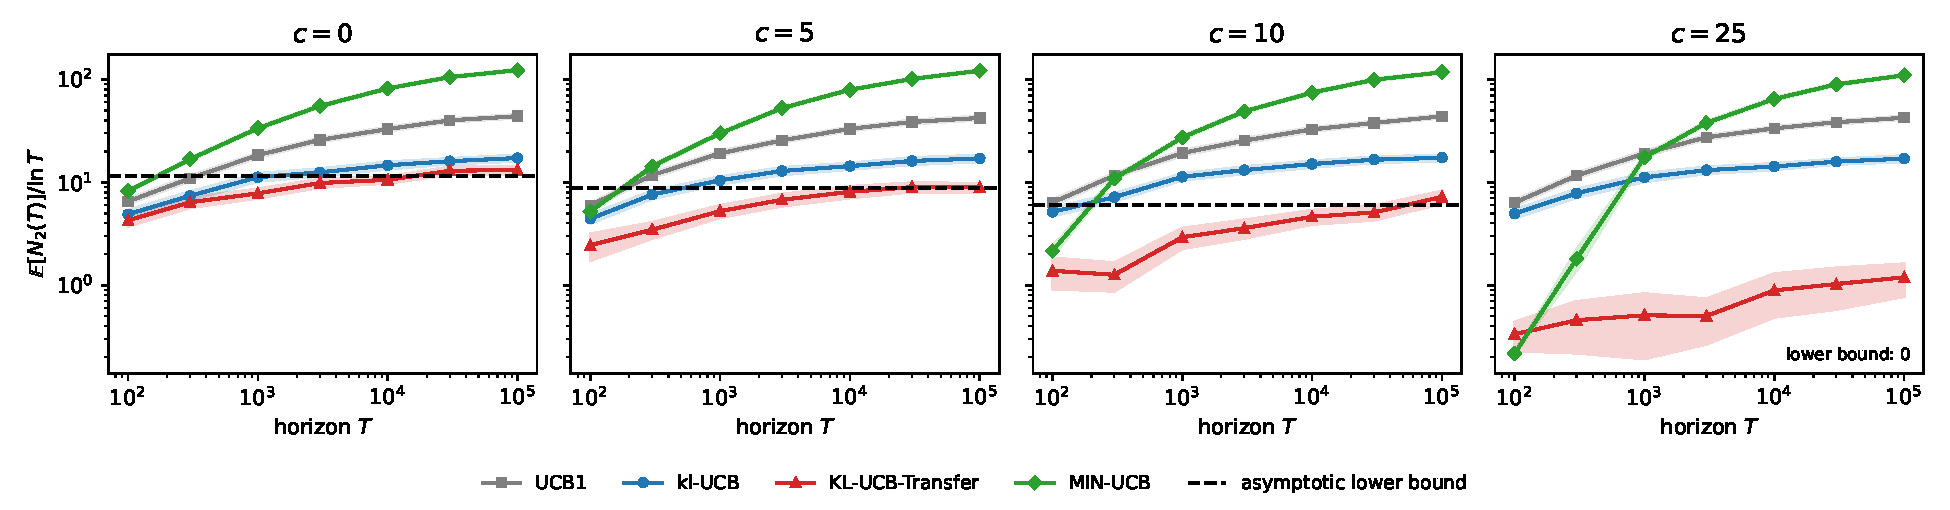
\includegraphics[width=\textwidth]{notebook/fig_counts.pdf}
\caption[Pulls of the suboptimal arm against the horizon]{Expected number of pulls of the suboptimal arm $2$, divided by $\ln T$, against the
horizon $T$, on the instance of Example~\ref{ex:bernoulli} with $\lfloor c\ln T\rfloor$ source
samples of arm $2$; mean of $100$ runs and $95\%$ confidence band, both axes logarithmic. Dashed: the asymptotic lower
bound $(1-c\Kp_2)_+/\Ka_2$ of Theorem~\ref{thm:main}.}\label{fig:counts}
\end{figure}

\paragraph{Interpretation of Figure~\ref{fig:counts}} At small horizons the curves may lie below
the asymptotic bound: for $c\in\{0,5\}$ all four learners are below it at $T=10^2$. This does not
contradict Theorem~\ref{thm:main}, which is a statement on the $\liminf$ as $T\to\infty$. The two
learners that ignore the source are in the four classes, so the bound that applies to them is the
classical $1/\Ka_2\approx11.47$ whatever $c$. Their curves do not depend on $c$ beyond the
confidence bands. They are below $11.47$ at $T=10^2$ (UCB1, every $c$; also at $T=3\cdot10^2$ for
$c=0$) and up to $T=10^3$ (kl-UCB), and above it from $T=10^3$ (UCB1) and $T=3\cdot10^3$ (kl-UCB)
on; at $T=10^5$ they are at about $44$ (UCB1) and $17.3$ (kl-UCB). KL-UCB-Transfer is the only learner whose counts stay
close to the bound as $c$ grows (its exploration function $\ln t+\ln\ln t$ is also smaller than
that of kl-UCB). At $T=10^5$ its ratio is about $13.2$, $8.9$, $7.2$ and $1.2$ for $c=0,5,10,25$,
against $11.47$, $8.77$, $6.06$ and $0$; with $c=25$ the source alone rules arm $2$ out. It is
below the bound up to $T=10^4$ for $c=0$ and $c=5$, and up to $T=3\cdot10^4$ for $c=10$; it
reaches the bound near $T=3\cdot10^4$ for $c=0$ and $c=5$, and between $3\cdot10^4$ and $10^5$
for $c=10$. MIN-UCB, run with the confidence level of its guarantee
($\log(2t/\delta_t)=\log(4Kt^3)$, and a sub-Gaussian constant $1$ while Bernoulli laws are
$1/4$-sub-Gaussian), pulls arm $2$ about seven times more than kl-UCB at $T=10^5$; its source helps
mostly at the smallest horizons, where the offline samples outnumber the online ones. The figure
shows finite-horizon counts of four learners: it illustrates the bound and its dependence on the
source size, and says nothing about its tightness for the whole class.

\paragraph{Degenerate cases} If the size rule is randomised, say $\Np^{(T)}_2=\lfloor c\ln T\rfloor$
with probability $1/2$ and $0$ otherwise (through $\Up_0$), then $\xr_2(T)\to c/2$ and the bound is
$(1-c\Kp_2/2)_+/\Ka_2$: the theorem sees only the expected size. At the boundary, with
$\nu'_2=\Ber(0.45)$ and the same $\nu,L$, we have $\Kp_2=\kl(0.45,0.45)=0$ and item (iii) gives the
classical constant $1/\Ka_2$ for every source strategy with $\limsup_T\xr_2(T)<\infty$. If
$\nu'_2=\Ber(0.5)$, then $\mean'_2>\ms-L_2$ and item (ii) gives $1/\Ka_2$ whatever the sizes. With
$\ms=1$, for instance $\nu_1=\Ber(1)$ and $\nu'_1=\Ber(0.9)$ (still in the four drift sets), the
bound is $0$.

\section{Conclusion and open questions}\label{sec:open}

We proved the lower bound of \citet[Theorem~2]{PMRM26} for every size rule with finite expected
sizes and for the four drift conditions, with the same constant; at the boundary
$\mean'_a=\ms-L_a$, the proof needs the expected sizes to be $O(\ln T)$. The method sees the
source only through the expected size, and the alternatives are fixed while $T\to\infty$. These
two limitations give the questions below.

\begin{openquestion}[The boundary with large sources]\label{oq:boundary}
\extends{D2}
Let $K\ge2$, $L\in(0,\infty)^K$, $\pi\in\Cl(\PcL)$, $(\nu,\nu')\in\PcL$ with $\ms<1$, a suboptimal
arm $a$ with $\mean'_a=\ms-L_a$, and a source strategy with $\E_{\nu'}[\Np^{(T)}_k]<\infty$ and
$\E_{\nu'}[\Np^{(T)}_a]/\ln T\to\infty$. Is
$\liminf_T\E[\Nc_a(T)]/\ln T\ge1/\Kinf(\nu_a,\ms)$, or is there a learner of $\Cl(\PcL)$ with
$\liminf_T\E[\Nc_a(T)]/\ln T<1/\Kinf(\nu_a,\ms)$ on such an instance? The method of
Theorem~\ref{thm:main} stops there: every admissible alternative has
$\m(\tilde\nu'_a)>\mean'_a$, hence $\KL(\nu'_a,\tilde\nu'_a)>0$, and the source term
$\E_{\nu'}[\Np^{(T)}_a]\KL(\nu'_a,\tilde\nu'_a)$ of Proposition~\ref{prop:fixed} exceeds $\ln T$
for every fixed alternative and large $T$. Moving the alternative with $T$ requires a consistency
that is uniform over alternatives, which $\Cl(\PcL)$ does not give.
\end{openquestion}

\begin{openquestion}[Fluctuations of the sizes driven by the source values]\label{oq:fluctuations}
\extends{D1}
Let $K\ge2$, $L\in(0,\infty)^K$, $\pi\in\Cl(\PcL)$, $(\nu,\nu')\in\PcL$, a suboptimal arm $a$
with $\mean'_a<\ms-L_a$, and a source strategy whose sizes do not use the randomisation $\Up$. Does
\begin{equation*}
\liminf_{T\to\infty}\frac{\E[\Nc_a(T)]}{\ln T}\ \ge\ \liminf_{T\to\infty}
\frac{\E_{\nu'}\big[\big(1-\Kp_a\,\Np^{(T)}_a/\ln T\big)_+\big]}{\Ka_a}
\end{equation*}
hold, a bound larger than that of Theorem~\ref{thm:main} by Jensen's inequality whenever the size
fluctuates on the scale $\ln T$? The change of measure of Proposition~\ref{prop:fixed} averages the
source term over the source data before any test variable is chosen, so it cannot see the
fluctuations; a change of measure conditional on the source data would see them, but under the
alternative the size rule changes the law of the sizes.
\end{openquestion}

% ---------------------------------------------------------------- appendices
\appendix

\section{Useful lemmas}\label{sec:cited}

In this section we present the results from other papers that we use: the fundamental inequality
with a source and two facts on size rules and learners from the setting paper of transfer bandits
\citep{INC-P003}, and the values of $\Kinf$ on laws on $[0,1]$ from the setting paper of batched
bandits \citep{INC-P006}.

The setting paper of transfer bandits \citep{INC-P003} uses the symbols of Section~\ref{sec:setting}; it writes
$\mathbb P$ and $\tilde{\mathbb P}$ for the two laws of the game and $\E_{\mathbb P}$ for the
expectation under $\mathbb P$.

\begin{lemma}[{From \citet[Corollary~4.2]{INC-P003}}]\label{cite:INC-P003-cor:fundamental}
\uses{def:laws, def:size-rule, def:game}
Let $K\ge2$, let $\Np$ be a size rule, $\pi$ a transfer learner, $T\in\N$, and
$(\nu,\nu'),(\tilde\nu,\tilde\nu')\in\Pc^K\times\Pc^K$ with $\E_{\nu'}[\Np_k]<\infty$ for every
arm $k$. Write $\PP:=\PP^T_{\nu',\Np,\nu,\pi}$ and $\tilde\PP:=\PP^T_{\tilde\nu',\Np,\tilde\nu,\pi}$.
For every measurable $Z:\Sd\times\Hs_T\to[0,1]$,
\begin{equation*}
\sum_{k=1}^K\E_{\nu'}[\Np_k]\KL(\nu'_k,\tilde\nu'_k)+\sum_{k=1}^K\E_{\PP}[\Nc_k(T)]\KL(\nu_k,\tilde\nu_k)
\ \ge\ \kl\big(\E_{\PP}[Z],\E_{\tilde\PP}[Z]\big),
\end{equation*}
the left-hand side in $[0,\infty]$ with $0\cdot\infty:=0$.
\end{lemma}

\begin{lemma}[{From \citet[Lemma~5.3]{INC-P003}}]\label{cite:INC-P003-lem:prior-game}
\uses{def:size-rule, def:prior-game}
(a) A constant map $\Np\equiv n^0\in\N^K$ is a size rule. (b) The counts $\Np$ of a prior bandit game
over $\Tp$ rounds (Definition~\ref{def:prior-game}) form a size rule, with $\Np_k\le\Tp$.
\end{lemma}

\begin{lemma}[{From \citet[Proposition~5.9]{INC-P003}}]\label{cite:INC-P003-prop:witness}
\uses{def:drift, def:class, def:game}
If a bandit algorithm $\sigma$ is consistent on $\Pc^K$ (for every $\nu\in\Pc^K$, every suboptimal
arm $k$ and every $\alpha>0$, $\E_{\sigma,\nu}[\Nc_k(T)]/T^\alpha\to0$), its source-ignoring learner $\pis$
belongs to $\Cl(\mathcal P_{\mathbf 1_K})$, where $\mathbf 1_K:=(1,\dots,1)$, hence to
$\Cl(\PcL)$ for every $L\in(0,\infty)^K$. The algorithm UCB of \citet{ACF02}, with parameter
$c_0>1/2$ (pull arm $t$ at
rounds $t\le K$, then at round $t>K$ an arm maximising
$\hat\mu_b(t-1)+\sqrt{2c_0\log t/\Nc_b(t-1)}$, with $\hat\mu_b(t-1)$ and $\Nc_b(t-1)$ the empirical
mean and the count of arm $b$ after $t-1$ rounds and ties broken by a fixed rule) is consistent on
$\Pc^K$; in particular $\Cl(\PcL)\ne\emptyset$.
\end{lemma}

The setting paper of transfer bandits \citep{INC-P003} writes $\mathcal C_L$ for our $\Cl(\PcL)$ and $c$ for our $c_0$;
with $c_0=1$, its UCB is the algorithm UCB1 of \citet[Figure~1]{ACF02}, up to $\log t$ in
place of $\log(t-1)$ in the index.

The setting paper of batched bandits \citep{INC-P006} writes $\mathcal M$ for the laws on $\R$ that
give mass $1$ to $[0,1]$, which we identify with $\Pc$, and $m$ for our $\m$; its $\KL$, $\kl$ and
$\mathcal K_{\inf}$ are ours (the same strict inequality on the mean, $\inf\emptyset:=\infty$).

\begin{lemma}[{From \citet[Proposition~4.2]{INC-P006}}]\label{cite:INC-P006-prop:kinf}
\uses{def:laws}
Let $P\in\Pc$ with mean $p:=\m(P)$, and let $\mu\in\R$. Then:
\begin{enumerate}[label=(\roman*)]
\item if $\mu\ge1$, then $\Kinf(P,\mu)=\infty$;
\item if $\mu<p$, then $\Kinf(P,\mu)=0$;
\item if $p\le\mu<1$, then
$2(\mu-p)^2\le\kl(p,\mu)\le\Kinf(P,\mu)\le\log\frac{1-p}{1-\mu}<\infty$;
\item if $P=\Ber(p)$ and $p\le\mu<1$, then $\Kinf(P,\mu)=\kl(p,\mu)$.
\end{enumerate}
\end{lemma}

Item (v) of that proposition, on instances, is not used. We also use, by name,
the convexity of $t\mapsto\ln t$ on $(0,\infty)$ (in the form $\ln((1-t)+tu)\ge t\ln u$), and the
Radon--Nikodym theorem.

\section{Proof of Proposition~\ref{prop:fixed}}\label{sec:proof-fixed}

The proposition follows from the fundamental inequality with a source
(Lemma~\ref{cite:INC-P003-cor:fundamental}) and an elementary bound on $\kl$, due to
\citet[(10)--(11)]{GMS19}, which we prove with its conventions at $q\in\{0,1\}$.

\begin{lemma}[A lower bound on the Bernoulli divergence]\label{lem:kl}
\uses{def:laws}
For all $p,q\in[0,1]$,
\begin{equation*}
\kl(p,q)\ \ge\ (1-p)\ln\frac{1}{1-q}-\ln2,
\end{equation*}
with $\ln(1/0):=\infty$ and $0\cdot\infty:=0$.
\end{lemma}
(see the proof in Subsection~\ref{sec:proof-kl}). As in \citet[(10)--(11)]{GMS19}; it is the folklore bound $\kl(p,q)\ge p\ln\frac1q-\ln2$
\citep[(10) and Section~7]{GMS20} applied to $(1-p,1-q)$; no contribution here.

\begin{proof}[Proof of Proposition~\ref{prop:fixed}]
\proves{prop:fixed}
\uses{def:laws, def:instance, def:size-rule, def:game, cite:INC-P003-cor:fundamental, lem:kl}
\emph{Setting.} Fix $\Np,\pi,T\ge1,a$ and the two pairs as in the statement; write
$\PP:=\PP^T_{\nu',\Np,\nu,\pi}$ and $\tilde\PP:=\PP^T_{\tilde\nu',\Np,\tilde\nu,\pi}$, so that
$\E=\E_{\PP}$ and $\tilde\E=\E_{\tilde\PP}$. \emph{Goal.}~\eqref{eq:fixed}.

\emph{Step 1: the left-hand side.} For $k\ne a$, $\tilde\nu_k=\nu_k$ and $\tilde\nu'_k=\nu'_k$, so
$\KL(\nu_k,\tilde\nu_k)=\KL(\nu'_k,\tilde\nu'_k)=0$, and the terms of $k\ne a$ in the left-hand
side of Lemma~\ref{cite:INC-P003-cor:fundamental} vanish (the expectations are finite: $\E_{\nu'}[\Np_k]<\infty$ by hypothesis and $\E[\Nc_k(T)]\le T$). That left-hand side is therefore the
left-hand side of~\eqref{eq:fixed}.

\emph{Step 2: the test variable.} Let $Z:=\Nc_a(T)/T$, a measurable function of $H_T$ with values in
$[0,1]$. Lemma~\ref{cite:INC-P003-cor:fundamental} (\emph{the fundamental inequality with a
source}), whose hypotheses are those of the proposition, gives
\begin{equation*}
\E_{\nu'}[\Np_a]\,\KL(\nu'_a,\tilde\nu'_a)+\E[\Nc_a(T)]\,\KL(\nu_a,\tilde\nu_a)
\ \ge\ \kl(p,q),\qquad p:=\frac{\E[\Nc_a(T)]}{T},\quad q:=\frac{\tilde\E[\Nc_a(T)]}{T}.
\end{equation*}

\emph{Step 3: the bound on $\kl$.} Since $\sum_k\Nc_k(T)=T$ under $\tilde\PP$,
\begin{equation*}
1-q=\frac{T-\tilde\E[\Nc_a(T)]}{T}=\frac{\sum_{k\ne a}\tilde\E[\Nc_k(T)]}{T},\qquad\text{so}\qquad
\ln\frac{1}{1-q}=\ln\frac{T}{\sum_{k\ne a}\tilde\E[\Nc_k(T)]},
\end{equation*}
both sides being $\infty$ when $\sum_{k\ne a}\tilde\E[\Nc_k(T)]=0$. Lemma~\ref{lem:kl} gives
$\kl(p,q)\ge(1-p)\ln\frac1{1-q}-\ln2$, which is the right-hand side of~\eqref{eq:fixed}. Combining
with Step 2 proves~\eqref{eq:fixed}.
\end{proof}

\subsection{Proof of Lemma~\ref{lem:kl}}\label{sec:proof-kl}

\begin{proof}
\proves{lem:kl}
\uses{def:laws}
\emph{Case $q\in(0,1)$.} Then $\kl(p,q)=p\ln\frac pq+(1-p)\ln\frac{1-p}{1-q}$, with $0\ln0:=0$,
and we split it as
\begin{align*}
\kl(p,q)&=\underbrace{p\ln p+(1-p)\ln(1-p)}_{\ge-\ln2}+\underbrace{p\ln\frac1q}_{\ge0}
+(1-p)\ln\frac1{1-q} &&\text{(expanding the logarithms)}\\
&\ge(1-p)\ln\frac1{1-q}-\ln2 &&\text{(the two braces, below)}.
\end{align*}
The first brace is minus the binary entropy of $p$, which is at most $\ln2$; the second is
non-negative since $q\le1$.

\emph{Case $q=0$.} The right-hand side is $(1-p)\cdot0-\ln2<0\le\kl(p,q)$.

\emph{Case $q=1$.} If $p<1$, then $\Ber(p)\not\ll\Ber(1)$, so $\kl(p,1)=\infty$ and the inequality
holds. If $p=1$, the right-hand side is $0\cdot\infty-\ln2=-\ln2<0=\kl(1,1)$.
\end{proof}

\section{Proof of Theorem~\ref{thm:main}}\label{sec:proof-main}

The proof combines Proposition~\ref{prop:fixed} with an alternative built by
Lemma~\ref{lem:alternative} and the rates given by consistency (Lemma~\ref{lem:rate}).
Lemma~\ref{lem:window} is the tool of Lemma~\ref{lem:alternative}.

\begin{lemma}[Near-optimal alternatives in a window]\label{lem:window}
\uses{def:laws, cite:INC-P006-prop:kinf}
Let $P\in\Pc$ and $\mu\in\R$ with $\m(P)\le\mu<1$, and let $\eta>0$ and $\varepsilon>0$. There is
$Q\in\Pc$ such that
\begin{equation*}
\mu<\m(Q)<\mu+\eta\qquad\text{and}\qquad\KL(P,Q)\le\Kinf(P,\mu)+\varepsilon .
\end{equation*}
\end{lemma}
(see the proof in Subsection~\ref{sec:proof-window}). This is \citet[Lemma~23]{PMRM26}, in a form
with a window of arbitrary width.

\begin{lemma}[The alternative stays in the drift set]\label{lem:alternative}
\uses{def:laws, def:instance, def:drift, lem:window, cite:INC-P006-prop:kinf}
Let $K\ge2$, $L\in(0,\infty)^K$, let $\mathcal I$ be one of $\PcL,\PcLs,\PcLo,\PcLos$, let
$(\nu,\nu')\in\mathcal I$ with $\ms<1$, let $a$ be a suboptimal arm and $\varepsilon>0$. There are
$Q,Q'\in\Pc$ such that the pair $(\tilde\nu,\tilde\nu')$ defined by
\begin{equation*}
\tilde\nu_a:=Q,\quad\tilde\nu'_a:=Q',\qquad \tilde\nu_k:=\nu_k,\quad\tilde\nu'_k:=\nu'_k\quad(k\ne a)
\end{equation*}
satisfies:
\begin{enumerate}[label=(\alph*)]
\item $(\tilde\nu,\tilde\nu')\in\mathcal I$;
\item $\m(Q)>\ms$; hence, under $\tilde\nu$, every arm $k\ne a$ is suboptimal;
\item $\KL(\nu_a,Q)\le\Kinf(\nu_a,\ms)+\varepsilon$ and $\KL(\nu'_a,Q')\le\Kinf(\nu'_a,\ms-L_a)+\varepsilon$;
\item if $\mean'_a>\ms-L_a$, then $Q'=\nu'_a$.
\end{enumerate}
\end{lemma}
(see the proof in Subsection~\ref{sec:proof-alternative}). The construction follows the two cases
of \citet[Appendix~E]{PMRM26}. In the second case we choose $Q'$ before $Q$; this replaces the
appeal of the source to the continuity of $\Kinf$ in its level \citep[Lemma~2 and
Theorems~7--8]{HT10} by a second use of Lemma~\ref{lem:window}, a simplification only.

\begin{lemma}[Rates from consistency]\label{lem:rate}
\uses{def:instance, def:size-rule, def:game, def:class}
Let $\mathcal I\subset\Pc^K\times\Pc^K$, $\pi\in\Cl(\mathcal I)$, $\rhos$ a source strategy, and
$a\in[K]$. If $(\nu,\nu')\in\mathcal I$ and $a$ is suboptimal for $\nu$, then
\begin{equation*}
\lim_{T\to\infty}\frac{\E_{\nu',\rhos,\nu,\pi}[\Nc_a(T)]}{T}=0 .
\end{equation*}
If $(\tilde\nu,\tilde\nu')\in\mathcal I$ and every arm $k\ne a$ is suboptimal for $\tilde\nu$, then
for every $\alpha\in(0,1)$ there is $T_0$ such that, for every $T\ge T_0$,
\begin{equation*}
\ln\frac{T}{\sum_{k\ne a}\E_{\tilde\nu',\rhos,\tilde\nu,\pi}[\Nc_k(T)]}\ \ge\ (1-\alpha)\ln T .
\end{equation*}
\end{lemma}
(see the proof in Subsection~\ref{sec:proof-rate}). As in the classical proof
\citep[Theorem~1]{GMS19}; no contribution here.

Two more lemmas organise the proof: the values of the constants, and the inequality obtained for
one alternative and all large horizons, before any limit is taken.

\begin{lemma}[The constants]\label{lem:constants}
\uses{def:laws, def:instance, cite:INC-P006-prop:kinf}
Let $K\ge2$, $\nu,\nu'\in\Pc^K$, $L\in(0,\infty)^K$, and $a$ a suboptimal arm of $\nu$, and let
$\Ka_a:=\Kinf(\nu_a,\ms)$ and $\Kp_a:=\Kinf(\nu'_a,\ms-L_a)$. Then $\Ka_a\in(0,\infty]$, with $\Ka_a<\infty$ if and only if $\ms<1$;
$\Kp_a\in[0,\infty)$; $\Kp_a>0$ if $\mean'_a<\ms-L_a$, and $\Kp_a=0$ if $\mean'_a\ge\ms-L_a$.
\end{lemma}
(see the proof in Subsection~\ref{sec:proof-constants}).

\begin{lemma}[One alternative, all large horizons]\label{lem:one-horizon}
\uses{def:laws, def:instance, def:size-rule, def:game, def:drift, def:class, prop:fixed, lem:alternative, lem:rate, lem:constants}
Let $K\ge2$, $L\in(0,\infty)^K$, let $\mathcal I$ be one of the four drift sets $\PcL$, $\PcLs$,
$\PcLo$, $\PcLos$, let $\pi\in\Cl(\mathcal I)$ and $(\nu,\nu')\in\mathcal I$ with $\ms<1$, let
$\rhos=(\Np^{(T)})_{T\ge1}$ be a source strategy with $\E_{\nu'}[\Np^{(T)}_k]<\infty$ for every arm
$k$ and every $T\ge1$, and let $a$ be a suboptimal arm of $\nu$. Let $\Ka_a:=\Kinf(\nu_a,\ms)$ and
$\Kp_a:=\Kinf(\nu'_a,\ms-L_a)$, write $\E[\cdot]:=\E_{\nu',\rhos,\nu,\pi}[\cdot]$ and, for $T\ge2$,
\begin{equation*}
\xr_a(T):=\frac{\E_{\nu'}[\Np^{(T)}_a]}{\ln T},\qquad
y(T):=\frac{\E[\Nc_a(T)]}{\ln T},\qquad p_T:=\frac{\E[\Nc_a(T)]}{T}.
\end{equation*}
Then $p_T\to0$, and for every $\varepsilon>0$ and every $\alpha\in(0,1)$ there are $\kappa'\in[0,\infty)$
and $T_0\ge2$ such that
\begin{equation*}
\kappa'\le\Kp_a+\varepsilon,\qquad \kappa'=0\ \text{ if }\mean'_a>\ms-L_a,
\end{equation*}
and, for every $T\ge T_0$,
\begin{equation}\label{eq:one-horizon-2}
y(T)\ \ge\ \frac{R_T}{\Ka_a+\varepsilon},\qquad
R_T:=(1-p_T)(1-\alpha)-\frac{\ln2}{\ln T}-\xr_a(T)\,\kappa' .
\end{equation}
\end{lemma}
(see the proof in Subsection~\ref{sec:proof-one-horizon}). Here $\kappa'$ is the divergence
$\KL(\nu'_a,\tilde\nu'_a)$ of the source law of arm $a$ to its alternative.

\begin{proof}[Proof of Theorem~\ref{thm:main}]
\proves{thm:main}
\uses{def:laws, def:instance, def:size-rule, def:game, def:drift, def:class, lem:constants, lem:one-horizon}
\emph{Idea.} Lemma~\ref{lem:one-horizon} gives, for each $(\varepsilon,\alpha)$, a lower bound on
$y(T)$ for large $T$, whose only term that may be large is the source term $\xr_a(T)\kappa'$. In each
case we bound that term, take the $\liminf$ in $T$ for fixed $(\varepsilon,\alpha)$, and then let
$\alpha\to0$ and $\varepsilon\to0$; the left-hand side does not depend on them.

\emph{Setting.} Fix $K,L,\mathcal I,\pi,(\nu,\nu'),\rhos$ and $a$ as in the statement, and use the
notation $y(T)$, $p_T$, $R_T$ of Lemma~\ref{lem:one-horizon}. \emph{Goal.} (i)--(iii); the claims
on $\Ka_a$ and $\Kp_a$ are Lemma~\ref{lem:constants} (\emph{the constants}).

\emph{Step 0: the case $\ms=1$.} Then $\Ka_a=\infty$ (Lemma~\ref{lem:constants}), and the right-hand
sides of~\eqref{eq:main-i} and~\eqref{eq:main-ii} are $0\le\liminf_Ty(T)$. From now on $\ms<1$, so
$\Ka_a\in(0,\infty)$, and Lemma~\ref{lem:one-horizon} applies to the data of the theorem (its
$\Ka_a$, $\Kp_a$ and $\xr_a(T)$ are those of the theorem). Fix $\varepsilon>0$ and
$\alpha\in(0,1)$, and let $\kappa'$ and $T_0$ be given by Lemma~\ref{lem:one-horizon} (\emph{one
alternative, all large horizons}).

\emph{Step 1: item (ii).} If $\mean'_a>\ms-L_a$, then $\kappa'=0$, so
$R_T=(1-p_T)(1-\alpha)-\ln2/\ln T\to1-\alpha$ since $p_T\to0$. By~\eqref{eq:one-horizon-2},
$\liminf_Ty(T)\ge(1-\alpha)/(\Ka_a+\varepsilon)$. Letting $\alpha\to0$ and $\varepsilon\to0$
gives~\eqref{eq:main-ii}.

\emph{Step 2: item (iii).} Let $\mean'_a=\ms-L_a$ and $C:=\limsup_T\xr_a(T)<\infty$. Then
$\Kp_a=0$ (Lemma~\ref{lem:constants}), so $\kappa'\le\varepsilon$, and there is $T_1\ge T_0$ with
$\xr_a(T)\le C+1$ for $T\ge T_1$. For $T\ge T_1$,
\begin{align*}
R_T&\ge(1-p_T)(1-\alpha)-\frac{\ln2}{\ln T}-(C+1)\varepsilon
&&\text{($0\le\xr_a(T)\le C+1$, $0\le\kappa'\le\varepsilon$)}\\
&\xrightarrow[T\to\infty]{}1-\alpha-(C+1)\varepsilon &&\text{($p_T\to0$, Lemma~\ref{lem:one-horizon})}.
\end{align*}
By~\eqref{eq:one-horizon-2}, $\liminf_Ty(T)\ge(1-\alpha-(C+1)\varepsilon)/(\Ka_a+\varepsilon)$, and
letting $\alpha\to0$, $\varepsilon\to0$ gives~\eqref{eq:main-ii}.

\emph{Step 3: item (i).} Let $\mean'_a<\ms-L_a$, so that $\Kp_a>0$ (Lemma~\ref{lem:constants}), and
let
\begin{equation*}
c:=\liminf_{T\to\infty}\big(1-\Kp_a\xr_a(T)\big)_+\in[0,1],
\end{equation*}
which depends neither on $\varepsilon$ nor on $\alpha$. If $c=0$, \eqref{eq:main-i} reads
$\liminf_Ty(T)\ge0$, which holds. Let $c>0$. There is $T_1\ge T_0$ such that
$(1-\Kp_a\xr_a(T))_+\ge c/2>0$ for $T\ge T_1$; for these $T$ the positive part is positive, so it
equals $1-\Kp_a\xr_a(T)$, and
\begin{equation*}
\xr_a(T)<\frac{1}{\Kp_a}\qquad(T\ge T_1).
\end{equation*}
Hence, for $T\ge T_1$, one step per line,
\begin{align*}
R_T&=(1-p_T)(1-\alpha)-\frac{\ln2}{\ln T}-\xr_a(T)\,\kappa'
&&\text{(definition of $R_T$, \eqref{eq:one-horizon-2})}\\
&\ge(1-p_T)(1-\alpha)-\frac{\ln2}{\ln T}-\xr_a(T)\Kp_a-\xr_a(T)\varepsilon
&&\text{($\kappa'\le\Kp_a+\varepsilon$, $\xr_a(T)\ge0$)}\\
&\ge1-\alpha-p_T-\frac{\ln2}{\ln T}-\Kp_a\xr_a(T)-\xr_a(T)\varepsilon
&&\text{(expanding; $\alpha p_T\ge0$)}\\
&\ge1-\Kp_a\xr_a(T)-\alpha-p_T-\frac{\ln2}{\ln T}-\frac{\varepsilon}{\Kp_a}
&&\text{($\xr_a(T)<1/\Kp_a$ for $T\ge T_1$)}\\
&=\big(1-\Kp_a\xr_a(T)\big)_+-\alpha-p_T-\frac{\ln2}{\ln T}-\frac{\varepsilon}{\Kp_a}
&&\text{($1-\Kp_a\xr_a(T)>0$ for $T\ge T_1$)}.
\end{align*}
Taking the $\liminf$ in $T$,
\begin{align*}
\liminf_{T\to\infty}y(T)&\ge\frac{\liminf_TR_T}{\Ka_a+\varepsilon}
&&\text{(\eqref{eq:one-horizon-2} for $T\ge T_0$)}\\
&\ge\frac{c-\alpha-\varepsilon/\Kp_a}{\Ka_a+\varepsilon}
&&\text{(chain above; $p_T\to0$; definition of $c$)}.
\end{align*}
The left-hand side and $c$ depend neither on $\alpha$ nor on $\varepsilon$, and $\Kp_a>0$ is fixed;
letting $\alpha\to0$ and $\varepsilon\to0$ gives $\liminf_Ty(T)\ge c/\Ka_a$, which
is~\eqref{eq:main-i}.
\end{proof}

\subsection{Proof of Lemma~\ref{lem:window}}\label{sec:proof-window}

\begin{proof}
\proves{lem:window}
\uses{def:laws, cite:INC-P006-prop:kinf}
\emph{Idea.} Take a near-optimal $Q_0$ in the definition of $\Kinf(P,\mu)$; its mean may be far
above $\mu$. Mixing it with $P$, whose mean is at most $\mu$, moves the mean continuously down into
the window, and convexity of the divergence in its second argument keeps $\KL(P,\cdot)$ below
$\KL(P,Q_0)$.

\emph{Step 1: a near-optimal law.} Since $\m(P)\le\mu<1$, $\Kinf(P,\mu)<\infty$
(Lemma~\ref{cite:INC-P006-prop:kinf}(iii)). By the definition of the infimum there is $Q_0\in\Pc$
with
\begin{equation*}
\m(Q_0)>\mu\qquad\text{and}\qquad\KL(P,Q_0)\le\Kinf(P,\mu)+\varepsilon<\infty .
\end{equation*}
If $\m(Q_0)<\mu+\eta$, then $Q:=Q_0$ works. Otherwise $\m(Q_0)\ge\mu+\eta$, and we go on.

\emph{Step 2: the mixture.} Let
\begin{equation*}
t:=\frac{\mu+\eta/2-\m(P)}{\m(Q_0)-\m(P)},\qquad Q:=(1-t)P+tQ_0 .
\end{equation*}
Since $\m(P)\le\mu<\mu+\eta/2<\mu+\eta\le\m(Q_0)$, we have $t\in(0,1)$, so $Q\in\Pc$, and by
linearity of the mean $\m(Q)=\m(P)+t(\m(Q_0)-\m(P))=\mu+\eta/2\in(\mu,\mu+\eta)$.

\emph{Step 3: the divergence.} Since $\KL(P,Q_0)<\infty$, $P\ll Q_0$; let $f:=dP/dQ_0$ (Radon--Nikodym
theorem). For every Borel set $A$, $P(A)=\int_Af\,dQ_0$ and $Q(A)=\int_A((1-t)f+t)\,dQ_0$, with
$(1-t)f+t\ge t>0$; hence $P\ll Q$ and
\begin{equation*}
\frac{dP}{dQ}=\frac{f}{(1-t)f+t}\qquad Q\text{-a.e.}
\end{equation*}
On the set $\{f>0\}$, which has $P$-measure $1$, we write $\ln\frac{dP}{dQ}=g$ with
$g:=-\ln\big((1-t)+t/f\big)$. Concavity of the logarithm, $\ln((1-t)\cdot1+t\cdot u)\ge(1-t)\ln1+t\ln u$
for $u=1/f>0$, gives
\begin{equation*}
g\ \le\ -t\ln\frac1f=t\ln f\qquad\text{on }\{f>0\}.
\end{equation*}
Moreover $g\le\ln\frac1{1-t}$, so the integral $\int g\,dP=\KL(P,Q)$ is well defined in
$[-\infty,\infty)$. The function $\ln f$ is $P$-integrable: its negative part satisfies
$\int(\ln f)^-\,dP=\int_{\{f<1\}}f\ln\frac1f\,dQ_0\le e^{-1}$, and $\int\ln f\,dP=\KL(P,Q_0)<\infty$.
Hence, one step per line,
\begin{align*}
\KL(P,Q)=\int g\,dP&\le t\int\ln f\,dP
&&\text{($g\le t\ln f$ on $\{f>0\}$, $P(f>0)=1$, $\ln f\in L^1(P)$)}\\
&=t\,\KL(P,Q_0)
&&\text{($\textstyle\int\ln f\,dP=\KL(P,Q_0)$)}\\
&\le\KL(P,Q_0)
&&\text{($t\le1$ and $\KL(P,Q_0)\ge0$)}\\
&\le\Kinf(P,\mu)+\varepsilon
&&\text{(the choice of $Q_0$, Step 1)}.
\end{align*}
Hence $Q$ has the two properties of the lemma.
\end{proof}

\subsection{Proof of Lemma~\ref{lem:alternative}}\label{sec:proof-alternative}

\begin{proof}
\proves{lem:alternative}
\uses{def:laws, def:instance, def:drift, lem:window, cite:INC-P006-prop:kinf}
\emph{Setting.} Fix $L,\mathcal I,(\nu,\nu')\in\mathcal I$ with $\ms<1$, a suboptimal arm $a$
and $\varepsilon>0$. Only arm $a$ changes, so for every $k\ne a$ the constraint of $\mathcal I$ on arm
$k$ holds for $(\tilde\nu,\tilde\nu')$ as for $(\nu,\nu')$. \emph{Goal.} Find $Q,Q'$ with (b)--(d)
and
\begin{equation}\label{eq:window-goal}
\text{(G1)}\quad\m(Q)-\m(Q')<L_a,\qquad\qquad
\text{(G2)}\quad\m(Q')-\m(Q)<L_a\ \text{ if }\mathcal I\in\{\PcL,\PcLs\}.
\end{equation}
Indeed, by Definition~\ref{def:drift}, the constraint on arm $a$ of a one-sided set ($\PcLo$ or
$\PcLos$) is implied by (G1), and that of a two-sided set ($\PcL$ or $\PcLs$) by (G1) and (G2)
together, which give $|\m(Q)-\m(Q')|<L_a$; so~\eqref{eq:window-goal} gives (a).

\emph{Case 1: $\mean'_a>\ms-L_a$.} Let $Q':=\nu'_a$, so that (d) holds and
$\KL(\nu'_a,Q')=0\le\Kinf(\nu'_a,\ms-L_a)+\varepsilon$. Let
\begin{equation*}
\eta:=\mean'_a+L_a-\ms>0 .
\end{equation*}
Lemma~\ref{lem:window} (\emph{near-optimal alternatives in a window}), applied with $P:=\nu_a$,
$\mu:=\ms$ (indeed $\m(\nu_a)=\mean_a<\ms<1$), this $\eta$ and $\varepsilon$, gives $Q$ with
\begin{equation*}
\ms<\m(Q)<\ms+\eta=\mean'_a+L_a\qquad\text{and}\qquad\KL(\nu_a,Q)\le\Kinf(\nu_a,\ms)+\varepsilon .
\end{equation*}
So (b) and (c) hold. For~\eqref{eq:window-goal}: (G1) holds, since
$\m(Q)-\m(Q')=\m(Q)-\mean'_a<L_a$ by the display. For (G2), let $\mathcal I$ be two-sided. Since
$(\nu,\nu')\in\mathcal I$, $\mean'_a-\mean_a\le L_a$, and since $\m(Q)>\ms>\mean_a$,
\begin{equation*}
\m(Q')-\m(Q)=\mean'_a-\m(Q)<\mean'_a-\mean_a\le L_a .
\end{equation*}
This gives (a).

\emph{Case 2: $\mean'_a\le\ms-L_a$.} Let $\lambda:=\ms-L_a$; then $\mean'_a\le\lambda<\ms<1$.
Lemma~\ref{lem:window} with $P:=\nu'_a$, $\mu:=\lambda$, $\eta:=L_a$ and $\varepsilon$ gives $Q'$
with
\begin{equation*}
\lambda<\m(Q')<\lambda+L_a=\ms\qquad\text{and}\qquad\KL(\nu'_a,Q')\le\Kinf(\nu'_a,\ms-L_a)+\varepsilon .
\end{equation*}
Then let
\begin{equation*}
\eta:=\m(Q')+L_a-\ms=\m(Q')-\lambda>0 .
\end{equation*}
Lemma~\ref{lem:window} with $P:=\nu_a$, $\mu:=\ms$, this $\eta$ and $\varepsilon$ gives $Q$ with
\begin{equation*}
\ms<\m(Q)<\ms+\eta=\m(Q')+L_a\qquad\text{and}\qquad\KL(\nu_a,Q)\le\Kinf(\nu_a,\ms)+\varepsilon .
\end{equation*}
So (b) and (c) hold, and (d) is void. For~\eqref{eq:window-goal}: $\m(Q)-\m(Q')<L_a$ by the last
display, and $\m(Q')-\m(Q)<\ms-\ms=0<L_a$ since $\m(Q')<\ms<\m(Q)$. This gives (a).

\emph{Item (b), second part.} For $k\ne a$, $\m(\tilde\nu_k)=\mean_k\le\ms<\m(Q)=\m(\tilde\nu_a)$, so the
largest mean of $\tilde\nu$ is $\m(Q)$, attained at $a$ only, and every $k\ne a$ is suboptimal for
$\tilde\nu$.
\end{proof}

\subsection{Proof of Lemma~\ref{lem:rate}}\label{sec:proof-rate}

\begin{proof}
\proves{lem:rate}
\uses{def:instance, def:size-rule, def:game, def:class}
\emph{First claim.} Apply Definition~\ref{def:class} to $(\nu,\nu')\in\mathcal I$, the strategy
$\rhos$, the suboptimal arm $a$ and $\alpha=1/2$: $\E_{\nu',\rhos,\nu,\pi}[\Nc_a(T)]/T^{1/2}\to0$,
so $\E_{\nu',\rhos,\nu,\pi}[\Nc_a(T)]/T\le T^{-1/2}\cdot\E_{\nu',\rhos,\nu,\pi}[\Nc_a(T)]/T^{1/2}\to0$.

\emph{Second claim.} Fix $\alpha\in(0,1)$. For each $k\ne a$, Definition~\ref{def:class} applied
to $(\tilde\nu,\tilde\nu')$, $\rhos$, the suboptimal arm $k$ and $\alpha$ gives
$\E_{\tilde\nu',\rhos,\tilde\nu,\pi}[\Nc_k(T)]/T^{\alpha}\to0$. Summing the $K-1$ limits, there is
$T_0$ such that
\begin{equation*}
\sum_{k\ne a}\E_{\tilde\nu',\rhos,\tilde\nu,\pi}[\Nc_k(T)]\ \le\ T^{\alpha}\qquad(T\ge T_0).
\end{equation*}
For these $T$, $\ln\big(T/\sum_{k\ne a}\E_{\tilde\nu',\rhos,\tilde\nu,\pi}[\Nc_k(T)]\big)\ge\ln(T/T^\alpha)=(1-\alpha)\ln T$
(the left-hand side being $\infty$ if the sum is $0$).
\end{proof}

\subsection{Proof of Lemma~\ref{lem:constants}}\label{sec:proof-constants}

\begin{proof}
\proves{lem:constants}
\uses{def:laws, def:instance, cite:INC-P006-prop:kinf}
\emph{The constant $\Ka_a$.} Since $\mean_a<\ms\le1$: if $\ms<1$,
Lemma~\ref{cite:INC-P006-prop:kinf}(iii) with $p=\mean_a$ and $\mu=\ms$ gives
$0<2(\ms-\mean_a)^2\le\Ka_a\le\ln\frac{1-\mean_a}{1-\ms}<\infty$; if $\ms=1$, item (i) gives
$\Ka_a=\infty$.

\emph{The constant $\Kp_a$.} The level $\ms-L_a$ is below $1$ since $\ms\le1$ and $L_a>0$. If
$\mean'_a>\ms-L_a$, Lemma~\ref{cite:INC-P006-prop:kinf}(ii) gives $\Kp_a=0$. If
$\mean'_a\le\ms-L_a$, item (iii) with $p=\mean'_a$ and $\mu=\ms-L_a$ gives
\begin{equation*}
2(\ms-L_a-\mean'_a)^2\ \le\ \Kp_a\ \le\ \ln\frac{1-\mean'_a}{1-(\ms-L_a)}<\infty,
\end{equation*}
so $\Kp_a>0$ when $\mean'_a<\ms-L_a$, and $\Kp_a=0$ when $\mean'_a=\ms-L_a$, where the upper bound is
$\ln1=0$.
\end{proof}

\subsection{Proof of Lemma~\ref{lem:one-horizon}}\label{sec:proof-one-horizon}

\begin{proof}
\proves{lem:one-horizon}
\uses{def:laws, def:instance, def:size-rule, def:game, def:drift, def:class, prop:fixed, lem:alternative, lem:rate, lem:constants}
\emph{Setting.} Fix the data of the statement. Since $\ms<1$, $\Ka_a\in(0,\infty)$
(Lemma~\ref{lem:constants}). \emph{Goal.} $p_T\to0$, then $\kappa'$, $T_0$
and~\eqref{eq:one-horizon-2}.

\emph{Step 1: the rate under $(\nu,\nu')$.} The first claim of Lemma~\ref{lem:rate} (\emph{rates
from consistency}), applied to $(\nu,\nu')\in\mathcal I$ and the suboptimal arm $a$, gives $p_T\to0$.

\emph{Step 2: one alternative.} Fix $\varepsilon>0$ and $\alpha\in(0,1)$. Let $Q,Q'$ and
$(\tilde\nu,\tilde\nu')$ be given by Lemma~\ref{lem:alternative} (\emph{the alternative stays in
the drift set}), and let
\begin{equation*}
\kappa:=\KL(\nu_a,Q),\qquad\kappa':=\KL(\nu'_a,Q').
\end{equation*}
By Lemma~\ref{lem:alternative}(b), $\m(Q)>\ms$, so $\kappa\ge\Ka_a>0$ by the definition of $\Kinf$;
by (c), $\kappa\le\Ka_a+\varepsilon$ and $\kappa'\le\Kp_a+\varepsilon<\infty$; by (d), $\kappa'=0$ if
$\mean'_a>\ms-L_a$. By (a), $(\tilde\nu,\tilde\nu')\in\mathcal I$, and by (b) every arm $k\ne a$ is
suboptimal for $\tilde\nu$. The second claim of Lemma~\ref{lem:rate} then gives some $T_0'$; let
$T_0:=\max(T_0',2)$, so that $\ln T>0$ for $T\ge T_0$. For $T\ge T_0$, with $\tilde\E[\cdot]:=\E_{\tilde\nu',\rhos,\tilde\nu,\pi}[\cdot]$,
\begin{equation*}
\ln\frac{T}{\sum_{k\ne a}\tilde\E[\Nc_k(T)]}\ \ge\ (1-\alpha)\ln T .
\end{equation*}

\emph{Step 3: the inequality for one horizon.} Let $T\ge T_0$. The pairs $(\nu,\nu')$ and
$(\tilde\nu,\tilde\nu')$ differ in arm $a$ only and $\E_{\nu'}[\Np^{(T)}_k]<\infty$ for every $k$,
so Proposition~\ref{prop:fixed} (\emph{change of measure with a source}) applies to the size rule
$\Np^{(T)}$, with $\E$ and $\tilde\E$ the expectations of the statement:
\begin{align*}
\E_{\nu'}[\Np^{(T)}_a]\,\kappa'+\E[\Nc_a(T)]\,\kappa
&\ge(1-p_T)\ln\frac{T}{\sum_{k\ne a}\tilde\E[\Nc_k(T)]}-\ln2
&& \text{(Proposition~\ref{prop:fixed})}\\
&\ge(1-p_T)(1-\alpha)\ln T-\ln2 && \text{(Step 2, and }1-p_T\ge0\text{)}.
\end{align*}
Both terms of the left-hand side are finite ($\E_{\nu'}[\Np^{(T)}_a]<\infty$, $\kappa'<\infty$,
$\E[\Nc_a(T)]\le T$, $\kappa\le\Ka_a+\varepsilon<\infty$), so the source term can be moved to the
right:
\begin{align*}
\E[\Nc_a(T)]\,\kappa
&\ge(1-p_T)(1-\alpha)\ln T-\ln2-\E_{\nu'}[\Np^{(T)}_a]\,\kappa'
&&\text{(the last display)}\\
&=R_T\ln T
&&\text{(definitions of $\xr_a(T)$ and $R_T$)}.
\end{align*}
Hence, for $T\ge T_0$,
\begin{align*}
y(T)&\ge\max\Big(\frac{R_T}{\kappa},0\Big)=\frac{(R_T)_+}{\kappa}
&&\text{(dividing by $\kappa\ln T>0$; $y(T)\ge0$)}\\
&\ge\frac{(R_T)_+}{\Ka_a+\varepsilon}
&&\text{($0<\kappa\le\Ka_a+\varepsilon$, $(R_T)_+\ge0$)}\\
&\ge\frac{R_T}{\Ka_a+\varepsilon}
&&\text{($(R_T)_+\ge R_T$)},
\end{align*}
which is~\eqref{eq:one-horizon-2}.
\end{proof}

\section{Proofs of the corollaries and of Lemma~\ref{lem:classes}}\label{sec:proofs-other}

This appendix derives the source theorem and the bound for concentrated sizes from
Theorem~\ref{thm:main}, and proves the inclusions between the drift sets and the classes used in
Section~\ref{sec:reduction} and Example~\ref{ex:bernoulli}. The bound for concentrated sizes uses
an elementary lemma on positive parts.

\begin{lemma}[Positive parts]\label{lem:positive-part}
(a) For all $a,b\in\R$, $a_+-b_+\le(a-b)_+$ and $|a_+-b_+|\le|a-b|$. (b) For all $\delta\in\R$,
$D\ge0$ and every integrable real random variable $N$,
\begin{equation*}
\big|\E[(\delta-DN)_+]-(\delta-D\,\E[N])_+\big|\ \le\ D\,\E\big|N-\E[N]\big| .
\end{equation*}
\end{lemma}
(see the proof in Subsection~\ref{sec:proof-positive-part}). As in \citet[Appendix~D]{PMRM26}; no
contribution here.

\subsection{Proof of Corollary~\ref{cor:source}}\label{sec:proof-cor}

\begin{proof}
\proves{cor:source}
\uses{def:laws, def:instance, def:size-rule, def:game, def:drift, def:class, def:prior-game, cite:INC-P003-lem:prior-game, thm:main}
\emph{Setting.} Fix $K,L,\pi,(\nu,\nu'),f$, the prior games and $a\ne1$ as in the statement.
\emph{Goal.} Items (i) and (ii).

\emph{Step 1: the hypotheses of Theorem~\ref{thm:main}.} By
Lemma~\ref{cite:INC-P003-lem:prior-game}(b), each $\Np^{(T)}$ is a size rule with
$\Np^{(T)}_k\le f(T)$, so $\rhos$ is a source strategy and $\E_{\nu'}[\Np^{(T)}_k]\le f(T)<\infty$
for every $k$ and $T$. Since $\mean_1>\mean_k$ for $k\ne1$, $\ms=\mean_1$ and $a$ is suboptimal. With
$\mathcal I:=\PcL$, all the hypotheses of Theorem~\ref{thm:main} hold, and its $\Ka_a$, $\Kp_a$,
$\xr_a(T)$ are $\Kinf(\nu_a,\mean_1)$, $\Kinf(\nu'_a,\mean_1-L_a)$ and
$\E_{\nu'}[\Np^{(T)}_a]/\ln T$.

\emph{Step 2: item (ii)} is Theorem~\ref{thm:main}(ii).

\emph{Step 3: item (i).} If $\mean'_a<\mean_1-L_a$, it is Theorem~\ref{thm:main}(i) (whose
conclusion holds without the hypothesis on the $\limsup$). If $\mean'_a=\mean_1-L_a$, then $\Kp_a=0$
by Theorem~\ref{thm:main}(iii), so the right-hand side of (i) is
$\liminf_T(1-0)_+/\Ka_a=1/\Ka_a$, and Theorem~\ref{thm:main}(iii), whose hypothesis
$\limsup_T\xr_a(T)<\infty$ is that of (i), gives $\liminf_T\E[\Nc_a(T)]/\ln T\ge1/\Ka_a$.
\end{proof}

\subsection{Proof of Lemma~\ref{lem:positive-part}}\label{sec:proof-positive-part}

\begin{proof}
\proves{lem:positive-part}
\uses{}
\emph{Item (a).} If $a\le0$, then $a_+-b_+=-b_+\le0\le(a-b)_+$. If $a>0$, then, since $b_+\ge b$,
\begin{equation*}
a_+-b_+=a-b_+\ \le\ a-b\ \le\ (a-b)_+ .
\end{equation*}
Exchanging $a$ and $b$ gives $b_+-a_+\le(b-a)_+$, so
$|a_+-b_+|\le\max\big((a-b)_+,(b-a)_+\big)=|a-b|$.

\emph{Item (b).} Let $g(n):=(\delta-Dn)_+$ for $n\in\R$. By (a), for all $n,m\in\R$,
\begin{equation*}
|g(n)-g(m)|\ \le\ |(\delta-Dn)-(\delta-Dm)|=D|n-m| .
\end{equation*}
Since $0\le g(N)\le|\delta|+D|N|$, $g(N)$ is integrable, and
\begin{align*}
\big|\E[g(N)]-g(\E[N])\big|&\le\E\big|g(N)-g(\E[N])\big|
&&\text{($|\E[X]|\le\E|X|$)}\\
&\le D\,\E\big|N-\E[N]\big| &&\text{(the Lipschitz bound above)},
\end{align*}
which is (b).
\end{proof}

\subsection{Proof of Corollary~\ref{cor:concentration}}\label{sec:proof-concentration}

\begin{proof}
\proves{cor:concentration}
\uses{def:laws, def:instance, def:size-rule, def:game, def:drift, def:class, thm:main, lem:positive-part}
\emph{Setting.} Assume the hypotheses of the corollary; write $N_T:=\Np^{(T)}_a$, a random variable
on $\Om$ under $\Pp_{\nu'}$, integrable by hypothesis, and, for $T\ge2$,
\begin{equation*}
b_T:=\E_{\nu'}\Big[\Big(1-\Kp_a\frac{N_T}{\ln T}\Big)_+\Big],\qquad
d_T:=\big(1-\Kp_a\,\xr_a(T)\big)_+ .
\end{equation*}
\emph{Goal.} $\liminf_T\E[\Nc_a(T)]/\ln T\ge\liminf_Tb_T/\Ka_a$.

\emph{Step 1: the two forms are close.} Lemma~\ref{lem:positive-part}(b) (\emph{positive parts}),
with $\delta:=1$, $D:=\Kp_a/\ln T\ge0$ (finite, by Theorem~\ref{thm:main}) and $N:=N_T$, gives,
since $\xr_a(T)=\E_{\nu'}[N_T]/\ln T$,
\begin{equation*}
|b_T-d_T|\ \le\ \Kp_a\,\frac{\E_{\nu'}|N_T-\E_{\nu'}[N_T]|}{\ln T}\ \xrightarrow[T\to\infty]{}\ 0 .
\end{equation*}
Hence $\liminf_Tb_T=\liminf_Td_T$.

\emph{Step 2: the lower bound.} By Theorem~\ref{thm:main}, items (i), (ii) and (iii) according to
the position of $\mean'_a$ with respect to $\ms-L_a$ (in (ii) and (iii), $\Kp_a=0$ and $d_T=1$), the
hypothesis of the corollary gives~\eqref{eq:main-unified}:
$\liminf_T\E[\Nc_a(T)]/\ln T\ge\liminf_Td_T/\Ka_a$. By Step 1 this is $\liminf_Tb_T/\Ka_a$.
\end{proof}

\subsection{Proof of Lemma~\ref{lem:classes}}\label{sec:proof-classes}

\begin{proof}
\proves{lem:classes}
\uses{def:drift, def:class, def:game, cite:INC-P003-prop:witness}
\emph{The sets.} For every arm $k$ and every pair: $|\mean_k-\mean'_k|<L_k$ implies
$|\mean_k-\mean'_k|\le L_k$ and $\mean_k-\mean'_k<L_k$; each of these implies
$\mean_k-\mean'_k\le L_k$. This gives the four inclusions.

\emph{The classes.} If $\mathcal I_1\subset\mathcal I_2$ and $\pi\in\Cl(\mathcal I_2)$, the
condition of Definition~\ref{def:class} holds for every pair of $\mathcal I_2$, hence for every pair
of $\mathcal I_1$, so $\pi\in\Cl(\mathcal I_1)$. Applied to the inclusions of the sets, this gives
the inclusions of the classes.

\emph{Source-ignoring learners.} Lemma~\ref{cite:INC-P003-prop:witness} gives
$\pis\in\Cl(\mathcal P_{\mathbf 1_K})$. Since means of laws on $[0,1]$ lie in $[0,1]$,
$|\mean_k-\mean'_k|\le1$ for every pair, so $\mathcal P_{\mathbf 1_K}=\Pc^K\times\Pc^K$, and
$\pis\in\Cl(\Pc^K\times\Pc^K)$. Every drift set is contained in $\Pc^K\times\Pc^K$, so, by the
inclusion of classes just proved, $\pis$ belongs to the four classes. The same lemma gives a bandit
algorithm consistent on $\Pc^K$ (UCB), so such algorithms exist.
\end{proof}

\section{Sources of the techniques}\label{sec:attribution}

For each technique of the proofs, where it is used and the earliest source we found.

\begin{center}
\begin{tabular}{@{}p{0.45\textwidth}p{0.47\textwidth}@{}}
\toprule
Technique (where) & Earliest source found \\
\midrule
\raggedright Change of measure with a data-processing inequality and the count as test variable
(Proposition~\ref{prop:fixed}) & for events at a stopping time, \citet[Lemma~1]{KCG16}; for a
$[0,1]$-valued test variable, \citet[(6), (10), Lemma~1]{GMS19}; for offline data collected by an
unknown adaptive policy, with the online laws, \citet[Appendix~B.1, (10)]{AJSS23}; with source laws
within a drift bound, \citet[Appendix~E, Lemmas~22 and~24]{PMRM26}, and for size rules the setting paper of transfer bandits \citep[Corollary~4.2]{INC-P003} \\[2pt]
\raggedright $\kl(p,q)\ge(1-p)\ln\frac1{1-q}-\ln2$ (Lemma~\ref{lem:kl}) & folklore \citep[Section~7]{GMS20}: their
(10), $\kl(p,q)\ge p\ln\frac1q-\ln2$, applied to $(1-p,1-q)$ \citep[(10)]{GMS20}; in bandit lower
bounds \citet[(10)--(11)]{GMS19} \\
\raggedright Mixing a near-optimal alternative with the original law to place its mean in a
window (Lemma~\ref{lem:window}) & \citet[Lemma~23]{PMRM26} \\
\raggedright Alternatives moving the target and the source law of one arm within the drift bound,
two cases (Lemma~\ref{lem:alternative}) & \citet[Appendix~E]{PMRM26}, whose second case uses the
continuity of $\Kinf$ in its level \citep[Lemma~2 and Theorems~7--8]{HT10}; choosing the source
alternative first, which avoids it, is a simplification \\
\raggedright Bounds $2(\mu-p)^2\le\kl(p,\mu)\le\Kinf(P,\mu)\le\ln\frac{1-p}{1-\mu}$
(Lemma~\ref{lem:constants}) & Pinsker's inequality for Bernoulli laws (history in
\citealp[Sections~3--4]{Rio23}) and data processing, as in \citet[(7)]{GHMS22}; mixing with a
Dirac mass, \citet[Appendix~B.1]{GHMS22}; in this form \citet[Proposition~4.2]{INC-P006} \\
\raggedright Lipschitz property of the positive part (Lemma~\ref{lem:positive-part},
Corollary~\ref{cor:concentration}) & \citet[Appendix~D]{PMRM26} \\
\raggedright Consistency under the alternative gives $\ln T$ evidence (Lemma~\ref{lem:rate},
Theorem~\ref{thm:main}) & \citet{LR85}; in this form \citet[Theorem~1]{GMS19} \\
\raggedright Restricting to the horizons where the bound is not trivial, to control the source term
without a growth hypothesis (Theorem~\ref{thm:main}, Step 3) & source not known \\
\bottomrule
\end{tabular}
\end{center}

\section{Notation}\label{sec:notation}

Every symbol is a link to its definition.

\begin{center}
\begin{tabular}{@{}p{0.34\textwidth}p{0.42\textwidth}p{0.18\textwidth}@{}}
\toprule
Symbol & Meaning & Defined in \\
\midrule
$\Pc$, $\m(P)$, $\Ber(p)$ & laws on $[0,1]$, mean, Bernoulli law & Definition~\ref{def:laws} \\
$\KL$, $\kl$ & divergence, Bernoulli divergence & Definition~\ref{def:laws} \\
$\Kinf(P,\mu)$ & smallest divergence to a law of mean $>\mu$ & Definition~\ref{def:laws} \\
$\mean_k$, $\mean'_k$, $\ms$ & target and source means, largest target mean & Definition~\ref{def:instance} \\
$\Om$, $\Up$, $\Xp_{k,j}$, $\Pp_{\nu'}$, $\Gc_n$ & source space, its coordinates and laws & Definition~\ref{def:size-rule} \\
$\Np$, $\rhos$ & size rule, source strategy & Definition~\ref{def:size-rule} \\
$\Dd$, $\Sd$ & source data and their space & Definition~\ref{def:size-rule} \\
$\Hs_t$, $\pis$, $\PP^T_{\nu',\Np,\nu,\pi}$, $\Nc_k(T)$ & histories, source-ignoring learner, law of the game, counts & Definition~\ref{def:game} \\
$\PcL$, $\PcLs$, $\PcLo$, $\PcLos$ & the four drift sets & Definition~\ref{def:drift} \\
$\Cl(\mathcal I)$ & learners consistent on $\mathcal I$ & Definition~\ref{def:class} \\
$\Tp$ & number of rounds of a prior bandit game & Definition~\ref{def:prior-game} \\
$\Ka_a$, $\Kp_a$, $\xr_a(T)$ & the constants and the normalised expected size & Theorem~\ref{thm:main} \\
\bottomrule
\end{tabular}
\end{center}

\bibliographystyle{plainnat}
\bibliography{refs,../../papers/library}

\end{document}
